\documentclass[a4paper,twoside]{article}

\usepackage{epsfig}
\usepackage{subcaption}
\usepackage{calc}
\usepackage{amssymb}
\usepackage{amstext}
\usepackage{amsmath}
\usepackage{amsthm}
\usepackage{multicol}
\usepackage{pslatex}
\usepackage{apalike}
\usepackage{algorithm2e}
\usepackage[bottom]{footmisc}
\usepackage{pdflscape}
\usepackage{SCITEPRESS}     % Please add other packages that you may need BEFORE the SCITEPRESS.sty package.




\begin{document}

\title{Deep Learning based Multi-Object Tracking for Crowd Detection, Tracking and Counting on Railway Platforms}

\author{\authorname{First Author Name\sup{1}\orcidAuthor{0000-0000-0000-0000}, Second Author Name\sup{1}\orcidAuthor{0000-0000-0000-0000} and Third Author Name\sup{2}\orcidAuthor{0000-0000-0000-0000}}
\affiliation{\sup{1}Institute of Problem Solving, XYZ University, My Street, MyTown, MyCountry}
\affiliation{\sup{2}Department of Computing, Main University, MySecondTown, MyCountry}
\email{\{first\_author, second\_author\}@ips.xyz.edu, third\_author@dc.mu.edu}}

\keywords{Crowd Counting, Multi-Object Tracking, DeepSORT, YOLO, Depth Estimation}

\abstract{We address real-time crowd detection, tracking, and unique counting on railway platforms under dense occlusions, strong perspective distortions, and camera motion during train arrivals. Building on a detect–track–count pipeline, we integrate a two-stage transfer-learned YOLOv11m head detector with an EfficientNet-B0 appearance encoder within a DeepSORT framework, and introduce a physics-constrained five-dimensional Kalman model (Phys-5D) that lifts image-plane kinematics to 3D via pinhole geometry while enforcing physically plausible depth dynamics. To overcome the brittleness of line-crossing under jitter and brief occlusions, we further propose a virtual counting band with persistence. On a representative MOT-format platform benchmark (20 videos, 18.5k frames), fine-tuning improves detection performance from mAP50 = 79.4\% / mAP50–95 = 54.7\% to 98.0\% / 81.6\%. Counting error is reduced to 2.24\% using our Phys-5D model, while maintaining an average of 39 identity switches. These results demonstrate that incorporating first-principles geometry and motion priors stabilizes trajectories and achieves state-of-the-art counting accuracy in safety-critical transportation scenarios, which in turn facilitates more effective train scheduling and enhances platform safety management.}

\onecolumn \maketitle \normalsize \setcounter{footnote}{0} \vfill

\section{\uppercase{Introduction}}
\label{sec:introduction}
Imagine a high-speed train approaching a busy platform. In the critical seconds before the train comes to a complete stop and doors open, it is operationally valuable for the driver and the onboard control system to anticipate the number of passengers waiting on the platform. Such foresight directly informs precise dispatching strategies and efficient boarding/alighting\cite{214,215,216}.

For railway operators, obtaining real-time situational awareness of platform crowds during train approach is essential to intelligent dispatch and proactive safety assurance\cite{214,215,216}. A vision system mounted on the train head can provide this “look-ahead” capability, transforming traditional passive platform monitoring into active, forward-looking risk assessment and operational decision-making.

\subsection{Objective}

Our objective is to use a camera mounted at the train head to detect, track, and uniquely count passengers on the platform in real time throughout the approach phase.

\subsection{Challenges}

\subsubsection{Challenge 1: Detection under extreme perspective changes and occlusion}
As the train approaches at speed, the camera undergoes large perspective changes: distant heads rapidly scale up and apparent motion is highly non-linear. Severe mutual occlusions inherent to dense crowds further degrade full-body detectors (e.g., YOLO variants), leading to instability and missed detections due to motion blur and heavy overlap\cite{29_kaur_systematic_2024,30_khan_passenger_2020,01_noauthor_deep_2024,66_zhang_bus_2020,33or34_li_lightweight_2023}.

\subsubsection{Solution 1: Robust head-based detection}
To mitigate these effects, we shift the detection target from full bodies to heads, which remain more visible at high density and under occlusion. Leveraging public datasets (CrowdHuman, Open Sensor Data for Rail 2023, RailEye3D) and our domain-specific RailwayPlatformCrowdHead dataset, we fine-tune a YOLOv11m detector via two-stage transfer learning\cite{shao2018crowdhuman,OpenSensorDataforRail2023,RailEye3D_Dataset}. The model is specialized for head cues from the train viewpoint and is robust to extreme scale variation and perspective distortion; the YOLO family is widely adopted for real-time detection\cite{02_noauthor_review_nodate,141}.

\subsubsection{Challenge 2: Tracking degradation due to ego-motion}
A central difficulty in multi-object tracking (MOT) is predicting targets’ next-frame states\cite{104,103}. Under fast ego-motion, classical motion models such as constant-velocity (8D) or constant-acceleration (12D) Kalman filters confound real target motion with apparent motion induced by camera movement, yielding physically inconsistent trajectories and frequent identity switches (ID switches).

\subsubsection{Solution 2: A physics-constrained model with ego-motion integration}
We propose Phys-5D, a five-dimensional Kalman variant that integrates the train’s ego-motion as prior knowledge in state prediction. Operating in a perspective-aware coordinate system with geometric constraints, Phys-5D decouples true target motion from apparent motion induced by camera advance. This significantly stabilizes trajectory predictions during rapid approach, reduces identity fragmentation, and preserves a compact state representation.

\subsubsection{Challenge 3: Converting dynamic tracks into reliable counts}
Even with stable tracking, converting rapidly evolving image-plane tracks into reliable, region-specific counts (e.g., per-car boarding zones) is nontrivial. Short occlusions and detection jitter can interrupt tracks, causing duplicates or misses for naive counting logic.

\subsubsection{Solution 3: Geography-anchored virtual counting zones}
We introduce geography-anchored virtual counting regions corresponding to real platform locations. Stabilized tracks are mapped to these zones with a temporal persistence window to absorb brief interruptions and positional jitter. 

\subsection{Results}
With domain-adaptive fine-tuning for the train-view setting, the head detector achieves a substantial accuracy gain: $mAP_{50}$ increases from 79.4\% to \textbf{98.0\%}, and $mAP_{50\text{--}95}$ from 54.7\% to \textbf{81.6\%}. On the \textbf{MOT-RPCH} benchmark built for this scenario, Phys-5D attains a \textbf{2.24\%} mean absolute percentage error (MAPE) in counting, surpassing constant-velocity (14.59\%) and constant-acceleration (6.99\%) baselines. It maintains \textbf{67\%} MOTA while substantially reducing identity switches. Combined with an EfficientNet-B0 appearance encoder, the system reliably restores identities after long occlusions from poles or other structures.

\subsection{Contributions}
In summary, our main contributions are:
\begin{itemize}
    \item We design a real-time, end-to-end \textbf{detect–track–analyze} pipeline tailored for train approach, enabling forward-looking platform perception onboard the train\cite{113,28_kaur_comprehensive_2023}.
    \item We propose a \textbf{Phys-5D Kalman filter} that incorporates physically grounded ego-motion constraints to address instability under strong perspective and camera motion.
    \item We release a new domain-specific dataset, \textbf{RailwayPlatformCrowdHead}, to facilitate head-based detection and crowd analytics from the train viewpoint.
    \item We demonstrate that combining physics-based motion modeling with deep visual representation yields \textbf{accurate, stable, and efficient} solutions for physically constrained vision tasks in transportation; for tracking-by-detection and DeepSORT foundations see\cite{132,211,212}.
\end{itemize}

\subsection{Preview}
Fig.~\ref{fig:intro_preview1} and Fig.~\ref{fig:intro_preview2} shows frames from a tracked video sequence, indicating currently tracked objects with their unique IDs and the unique-ID count from the virtual counting zone displayed at the bottom-left.
\begin{figure}[htbp]
    \centering
    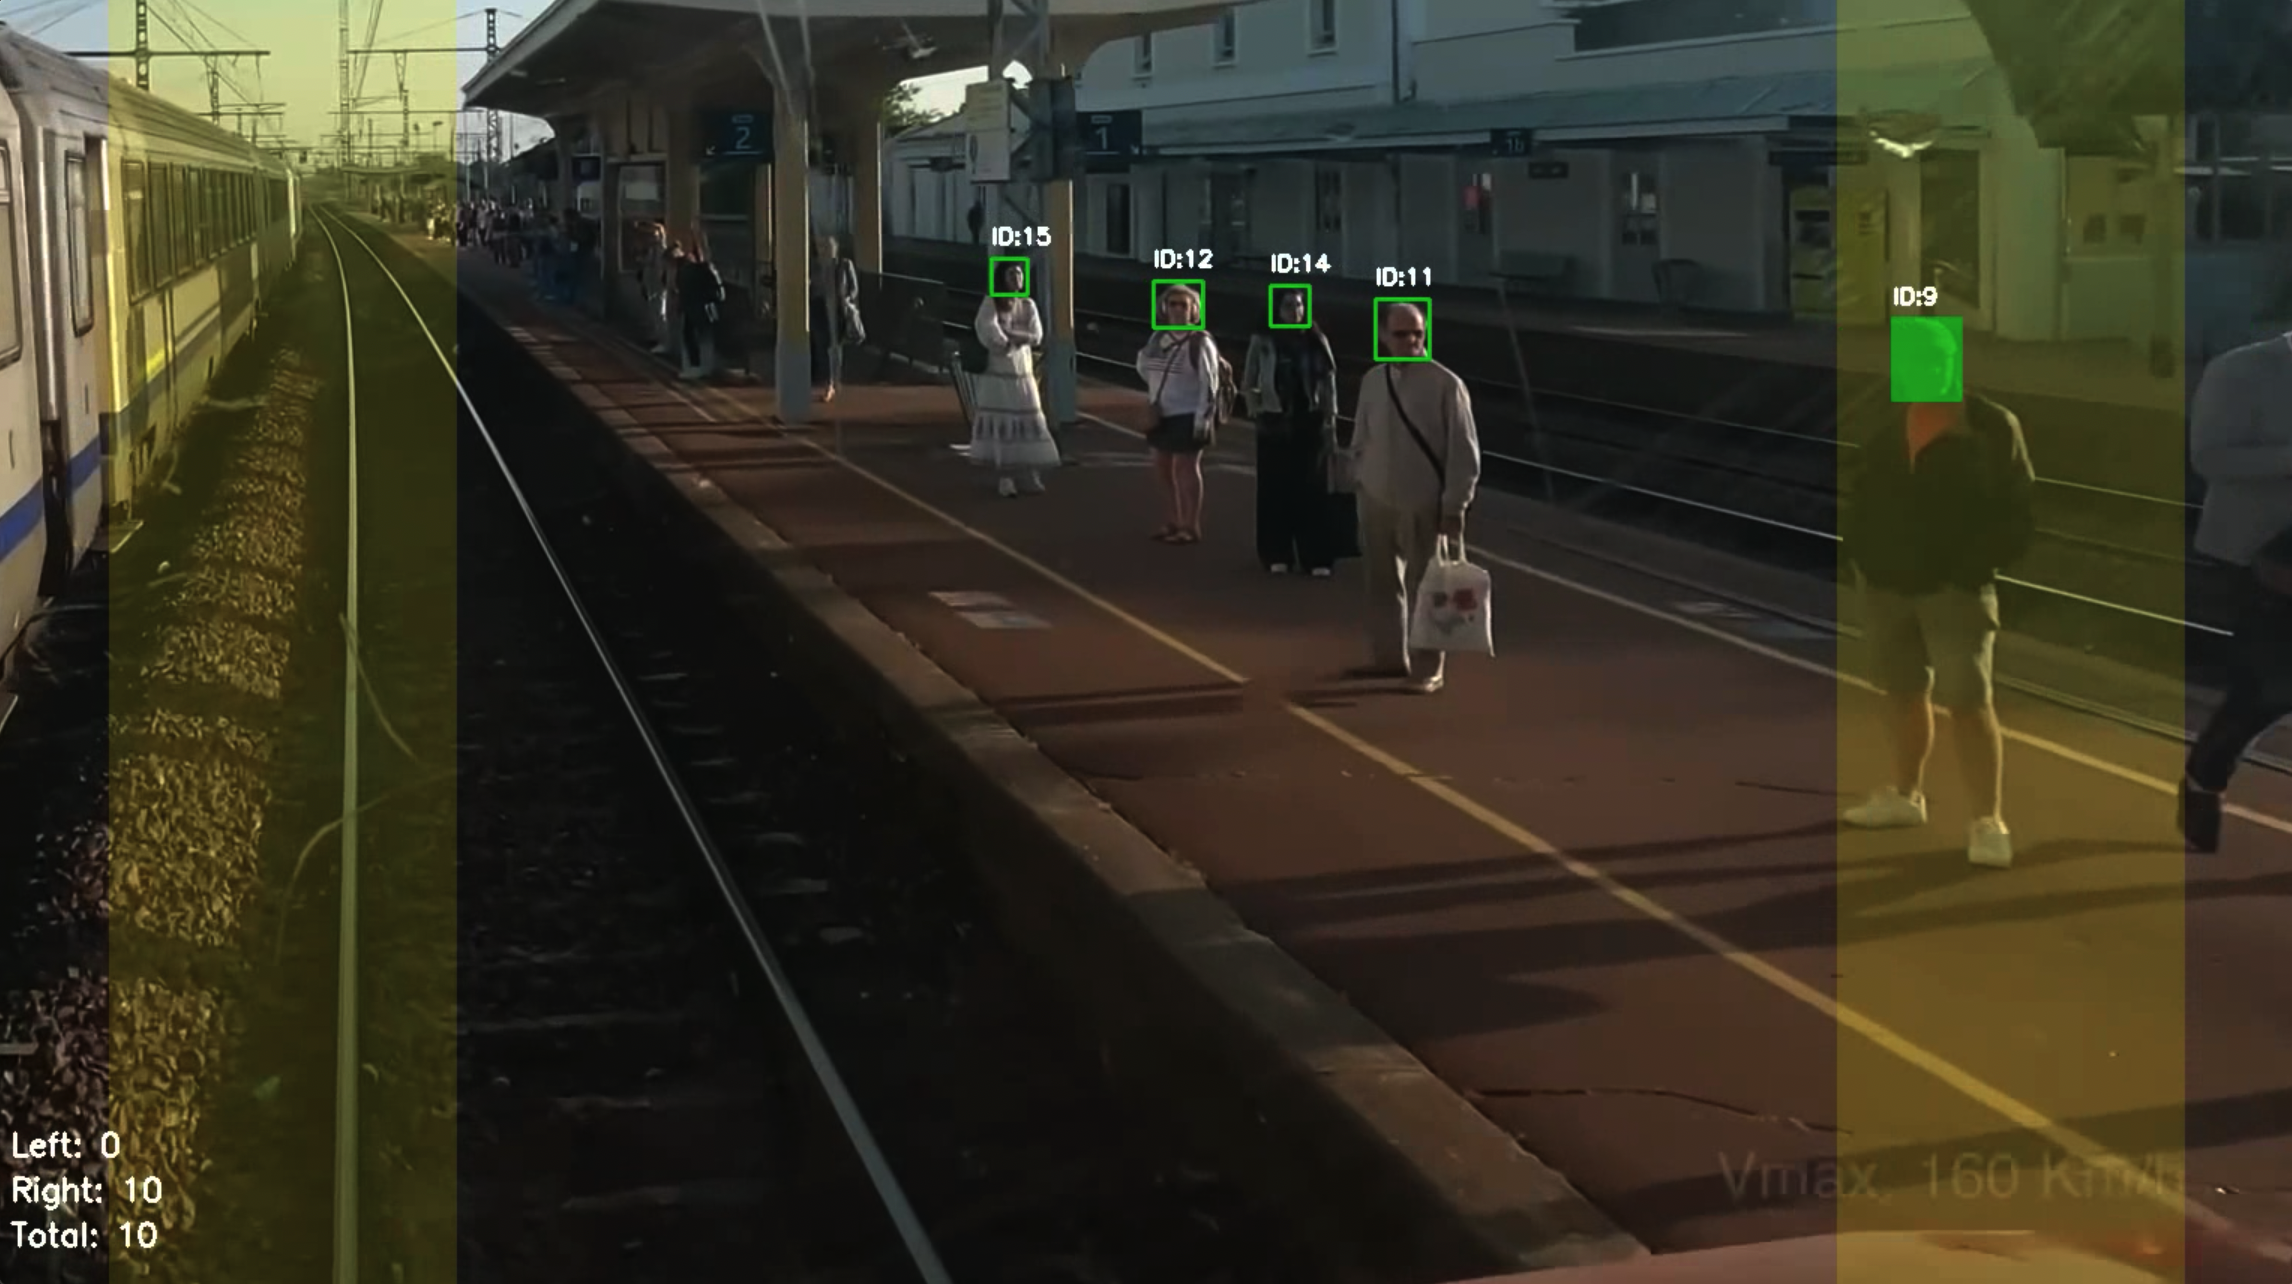
\includegraphics[width=0.49\textwidth]{pictures/Phys5Dframedeomo.png}  
    \caption{Frames from a tracked video sequence. Each bounding box is annotated with a unique track ID:9,11,14,12,15; the bottom-left overlay shows the unique-ID count(Total:10) from the virtual counting zone(yellow area).}
    \label{fig:intro_preview1}
\end{figure}

\begin{figure}[htbp]
    \centering
    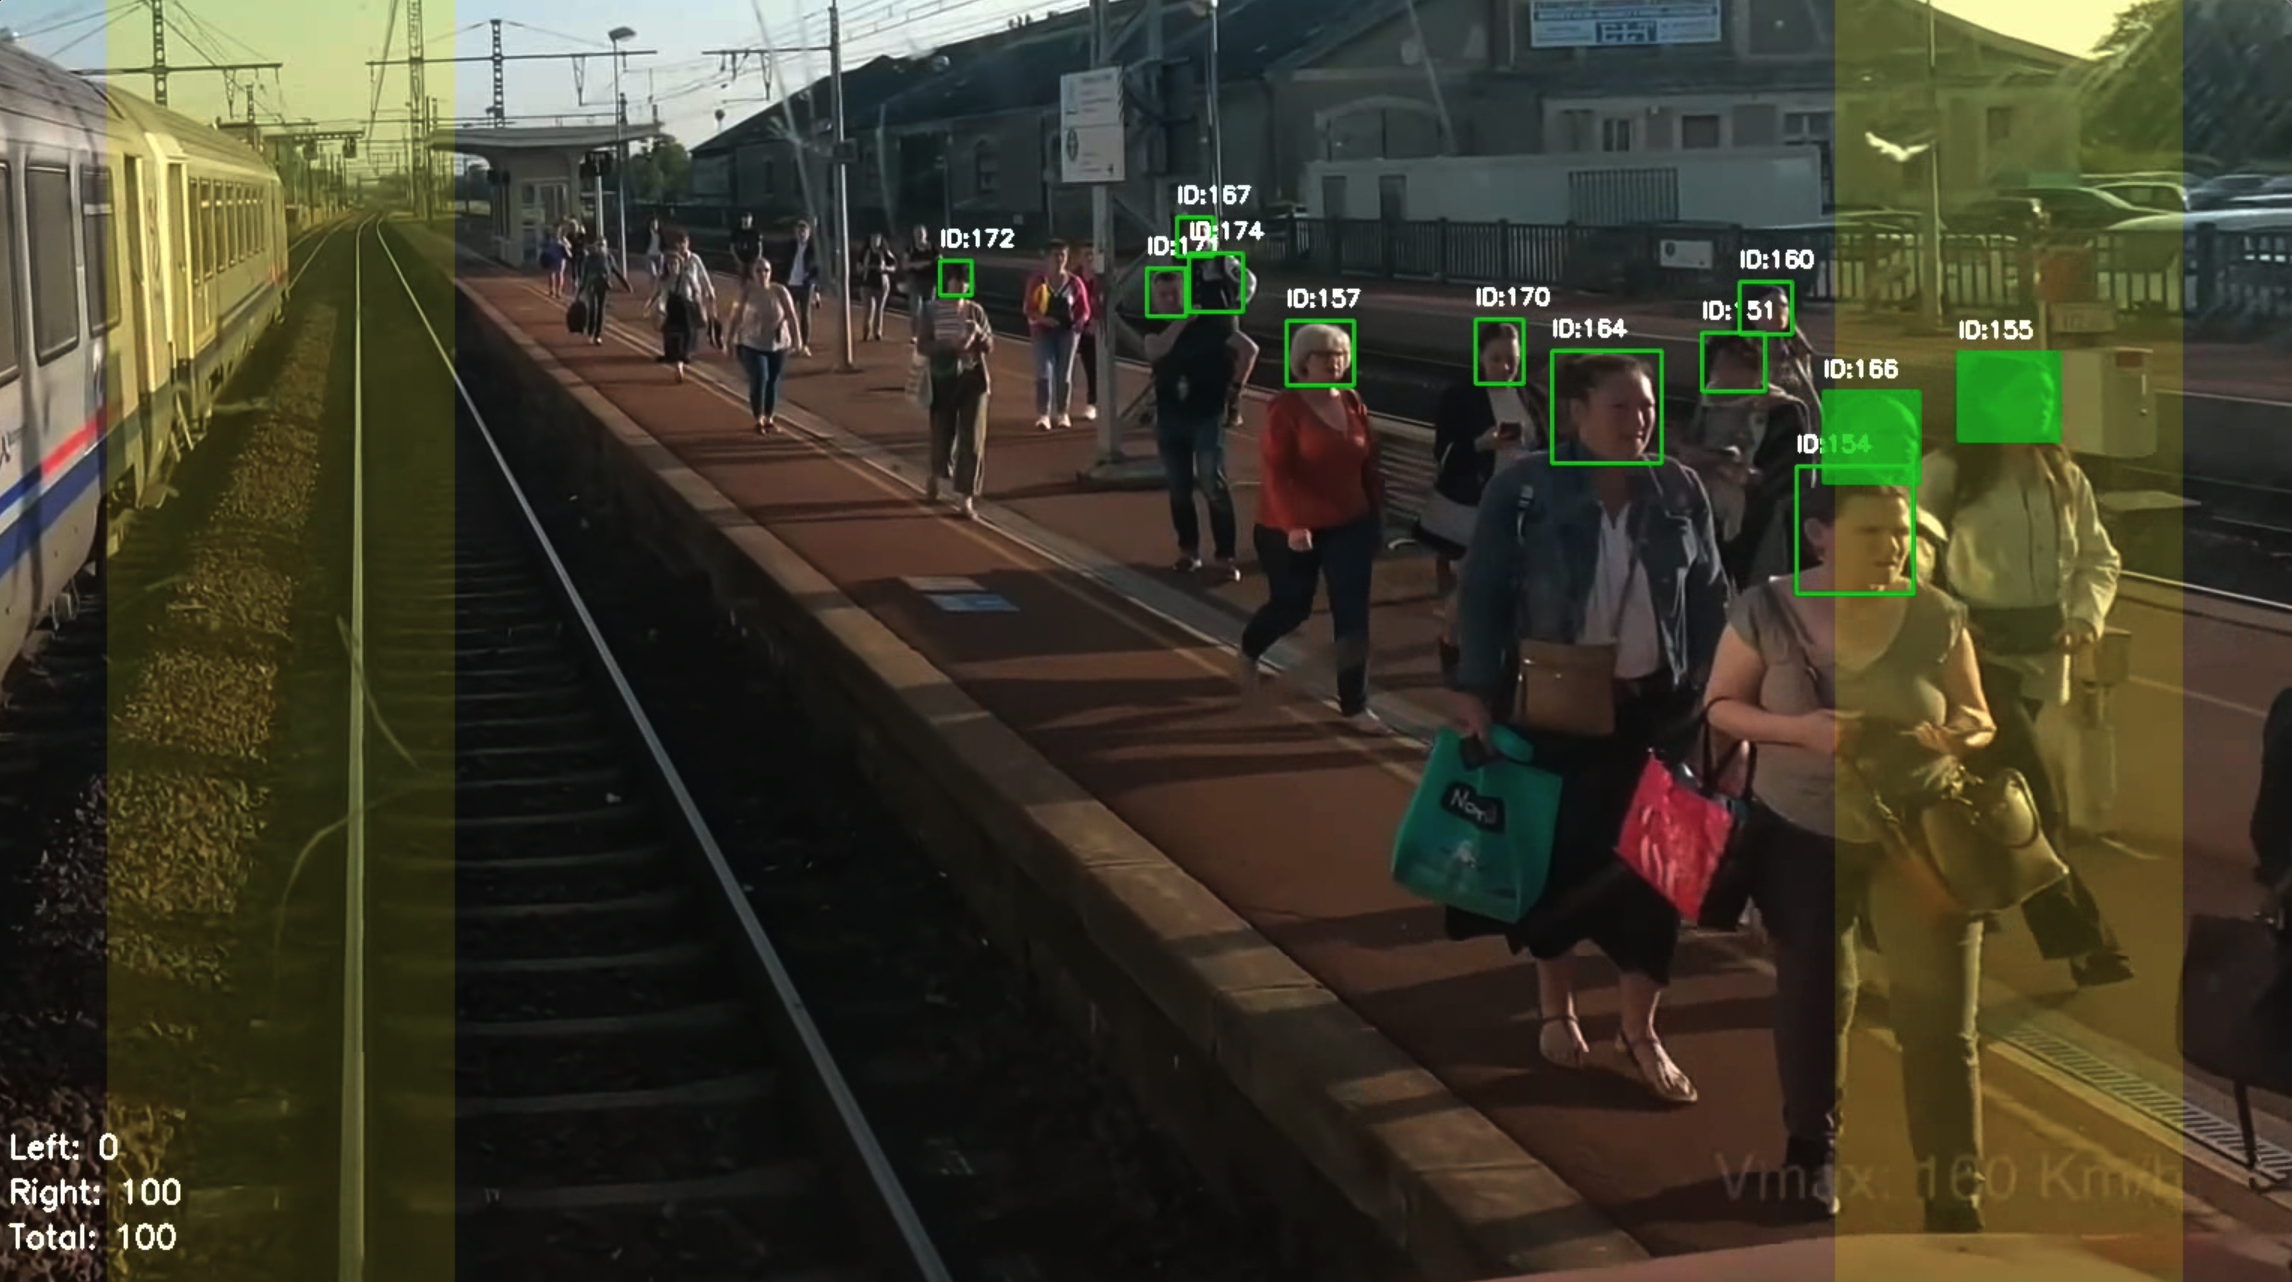
\includegraphics[width=0.49\textwidth]{pictures/Phys5Dframedeomo2.png}  
    \caption{Frames from a tracked video sequence. Each bounding box is annotated with a unique track ID:154,155,166 ...; the bottom-left overlay shows the unique-ID count(Total:100) from the virtual counting zone(yellow area).}
    \label{fig:intro_preview2}
\end{figure}



\section{\uppercase{Related Work}}
\label{sec:related_work}
Passenger detection and counting have evolved from handcrafted visual models to end-to-end deep learning frameworks. This section reviews related work in three domains: traditional methods, deep learning–based detection and tracking, and railway-specific crowd analysis.

\subsection{Traditional Methods}
Before deep learning dominated the field, crowd and passenger counting relied on handcrafted features and shallow models. Techniques such as Histogram of Oriented Gradients (HOG) and Hough transform were applied to detect passengers in bus or platform images \cite{30_khan_passenger_2020,73_Huofu}. While computationally efficient, these classical approaches were highly sensitive to illumination, perspective, and occlusion, resulting in poor generalization to crowded or dynamic scenes. Regression-based models that estimated global crowd density from low-level features \cite{zhang2016single,li2018csrnet} improved robustness but still failed to capture fine-grained individual localization.

\subsection{Deep Learning for Crowd Detection and Counting}
The advent of convolutional neural networks (CNNs) enabled the transition from feature engineering to feature learning. Early deep regression networks \cite{zhang2016single,li2018csrnet} predicted pixel-wise density maps, providing accurate crowd estimates in surveillance footage. However, density-based methods lose instance-level information required for multi-object tracking and identity consistency.  
Object detection frameworks such as Faster R-CNN and YOLO series \cite{redmon2016you,bochkovskiy2020yolov4,74_yolo11_Jocher_Ultralytics_YOLO_2023} addressed this issue by enabling explicit localization. They have since been adapted to head detection tasks \cite{shao2018crowdhuman}, which are more robust in dense or occluded environments. Recent transformer-based detectors further improved long-range context modeling but typically require large datasets and high computational cost, limiting deployment in real-time transportation monitoring.

\subsection{Multi-Object Tracking and Re-Identification}
Multi-object tracking (MOT) extends detection into temporal association. Early online trackers combine Kalman filtering with Hungarian matching, achieving real-time performance\cite{220}. Later works introduced appearance models and motion prediction enhancements, reducing identity switches in crowded scenarios\cite{211}. Appearance-based re-identification (Re-ID) has become essential for maintaining consistent identities across frames\cite{221_OccludedPersonReIdentification_ning2023}. Networks based on EfficientNet and ResNet backbones extract discriminative embeddings that support robust association even under partial occlusions\cite{222,223_Luo_2020}. Despite these advances, most trackers assume a fixed camera and constant-velocity motion model, which breaks down in scenes with strong perspective variation or moving cameras—typical conditions for railway surveillance.

\subsection{Crowd Counting in Transportation Scenarios}
Compared with generic crowd scenes, railway platforms present unique challenges: frequent partial occlusions, fast camera motion, and pronounced scale variation. While vehicle- or station-level passenger analytics have been studied \cite{di_gennaro_hum-card_2024,OpenSensorDataforRail2023}, most approaches rely on full-body detection, making them susceptible to mutual occlusion.  
Recent studies have highlighted the advantages of head-based counting \cite{shao2018crowdhuman}, yet publicly available datasets remain limited and lack domain diversity for railway applications. The absence of unified benchmarks and physically grounded motion models further constrains reproducibility and cross-domain generalization.

\subsection{Summary and Research Gap}
In summary, while deep detection and tracking frameworks have achieved impressive accuracy in general crowd scenes, their performance degrades under railway-specific constraints: nonstationary cameras, narrow viewing angles, and dense human occlusion. Traditional constant-velocity Kalman filters fail to model perspective geometry, causing instability in trajectory estimation and erroneous counts. Moreover, few works explicitly address robust, unique counting—distinguishing repeated entries and exits—from a physically constrained motion perspective.  
This motivates our work: an integrated detect–track–count system that combines head-based detection, appearance-aware re-identification, and a novel physics-constrained Kalman model designed to handle perspective distortion and physically plausible motion in real-time railway surveillance.




\section{\uppercase{Methods}}
\label{sec:methods}
This section presents our complete method for accurate crowd counting on railway platforms. We propose a detect–track–count pipeline that combines YOLOv11m head detection, EfficientNet-B0-based ReID feature extraction, and a physics-constrained 3D Kalman filter for robust multi-object tracking. Our key innovation is the Phys-5D physics-constrained tracker that leverages camera geometry and scene priors to stabilize identity consistency and achieve superior counting accuracy.

\subsection{System Architecture}

We tackle platform crowd counting with a detect–track–count pipeline tailored to station-arrival videos with dense occlusions and strong perspective effects. The system integrates YOLOv11-based object detection, EfficientNet-B0 ReID feature extraction, and a 3D physical Kalman filter for robust pedestrian tracking.

\begin{figure}[htbp]
    \centering
    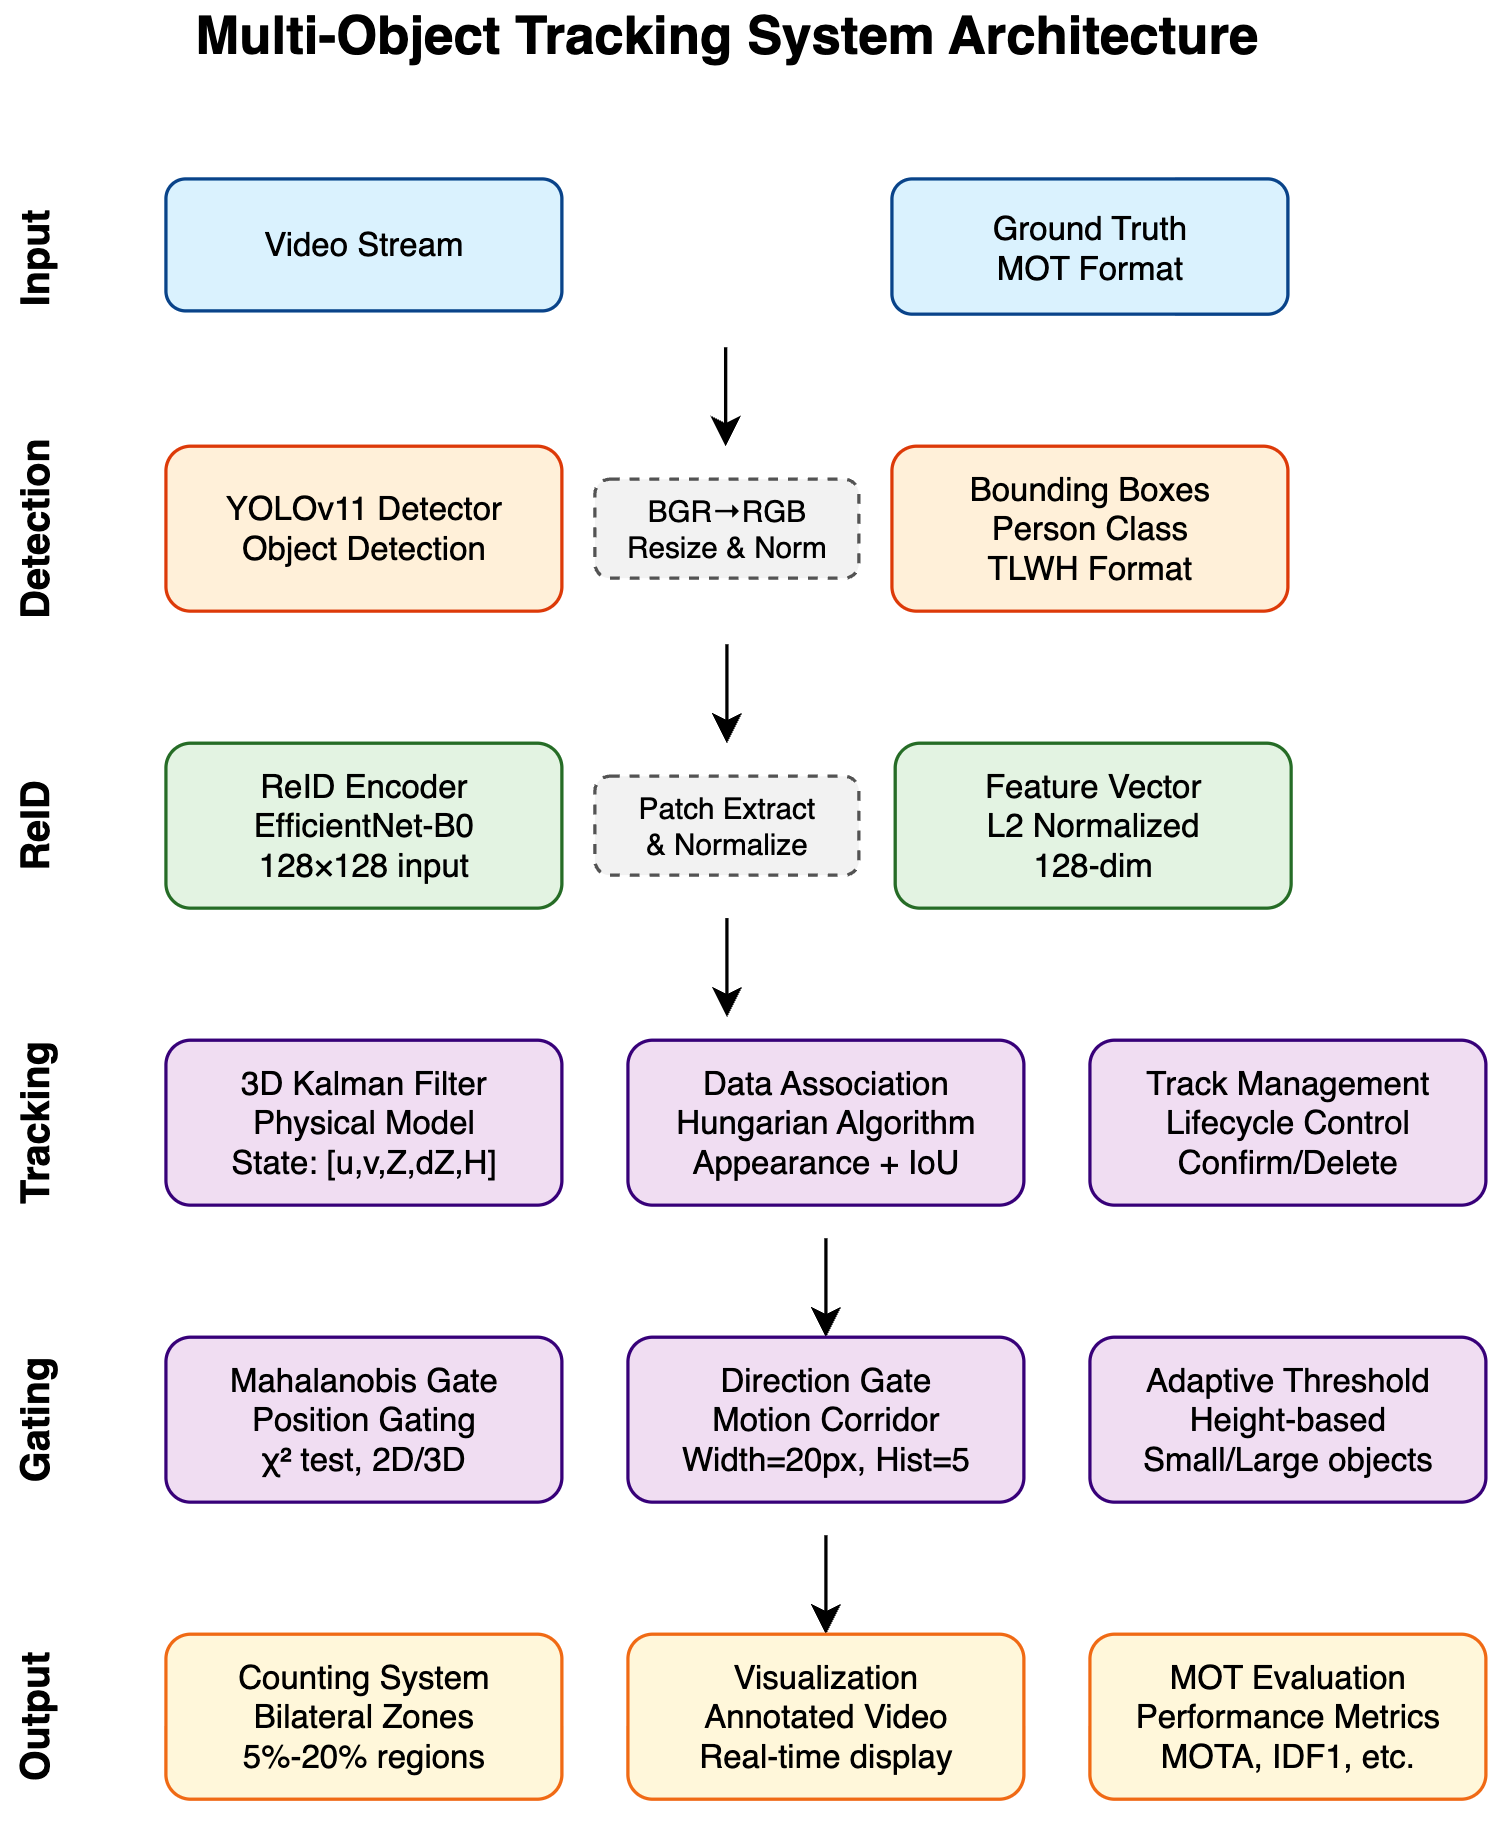
\includegraphics[width=0.49\textwidth]{pictures/OurMulti-ObjectTrackingSystemArchitecture.png}
    \caption{Overall Multi-object Tracking System Architecture. The system integrates YOLOv11-based object detection, EfficientNet-B0 ReID feature extraction, and a 3D physical Kalman filter for robust pedestrian tracking. The pipeline consists of five modules: (1) Input, which includes video streams and ground-truth annotations in MOT format; (2) Detection, where YOLOv11 detects pedestrian bounding boxes (TLWH format); (3) ReID, which extracts 128-dimensional L2-normalized feature vectors using an EfficientNet-B0 encoder; (4) Tracking and Gating, which performs data association via a Hungarian algorithm combining appearance and IoU metrics, managed by a 3D Kalman filter with state variables [u, v, z, dZ, H] and multiple gating strategies including Mahalanobis distance, directional motion corridors, and adaptive thresholds; and (5) Output, which provides bilateral-zone counting, annotated visualization, and MOTChallenge performance evaluation (MOTA, IDF1, etc.). This modular architecture ensures accurate, stable, and interpretable tracking across video sequences.}
    \label{fig:OurMOTSystemArchitecture}
\end{figure}


\subsection{Dataset and Preprocessing}

We constructed a comprehensive multi-modal dataset ecosystem for our experiments. The dataset includes:

\textbf{Training Data:} We use CrowdHuman dataset \cite{shao2018crowdhuman} (15,000 training images, 4,370 validation images) for pre-training, followed by fine-tuning on 2,000 annotated railway platform images from three sources: Open Sensor Data for Rail 2023 \cite{OpenSensorDataforRail2023} (20 images, 180 instances), RailEye3D Dataset \cite{RailEye3D_Dataset} (320 images, 1,221 instances), and our RailwayPlatformCrowd Dataset (1,660 images, 5,831 instances).

\textbf{Evaluation Dataset:} For comprehensive evaluation, we constructed the MOT-RailwayPlatformCrowdHead (MOT-RPCH) dataset containing 27 video sequences with 24,788 frames, 89,087 bounding boxes, and 885 unique human head identities. We select a representative subset of 20 video sequences for evaluation, spanning multiple resolutions (1536×864 to 2304×1296), frame rates (25, 29.97, 59.94 FPS), and target scales, totaling 18,548 frames, 647 identities, and 73,799 bounding boxes.

\subsection{YOLO and DeepSORT: Background and Limitations}

\textbf{YOLO (You Only Look Once):} YOLO \cite{redmon2016you} revolutionized object detection by formulating detection as a regression problem, enabling real-time performance through single-pass inference. However, in crowded railway platform scenarios, YOLO faces significant challenges: (1) severe occlusions between pedestrians degrade detection accuracy, (2) small head targets are difficult to localize consistently, and (3) perspective effects cause scale variations that confuse standard detection approaches.

\textbf{DeepSORT:} DeepSORT \cite{211} extends SORT by incorporating deep appearance embeddings with motion information through a Kalman filter. While effective for general tracking scenarios, DeepSORT has inherent limitations in railway platform contexts: (1) the standard 8D constant-velocity model assumes linear motion, which fails under train deceleration, (2) 2D image-plane tracking cannot leverage 3D scene geometry, and (3) identity switches increase dramatically under dense occlusions and perspective effects.

These limitations motivate our physics-constrained 3D tracking approach that explicitly models train deceleration and leverages camera geometry for improved accuracy.

\subsection{YOLOv11 Head Detection}

We adopt YOLOv11m for head detection to reduce occlusion-induced misses and stabilize localization for small targets. Our approach uses two-stage transfer learning:

\textbf{Stage 1:} Pre-training on CrowdHuman dataset achieves mAP50=79.4\% and mAP50–95=54.7\%.

\textbf{Stage 2:} Fine-tuning with backbone=10 frozen on railway platform head images achieves mAP50=98.0\% (+18.6 points) and mAP50–95=81.6\% (+26.9 points).

The detector uses SGD optimizer (lr=0.01, momentum=0.937, weight decay=0.0005), cosine annealing scheduler, and mixed precision training. Inference thresholds are set to confidence=0.5, IoU=0.7, input size=640×640.

\subsection{DeepSORT with EfficientNet-B0 ReID}

We extend the standard DeepSORT framework with EfficientNet-B0 for appearance feature extraction. The ReID model is trained on 7 video sequences with 238 tracked identities from our MOT-RPCH dataset. Through comprehensive input size ablation experiments, we select 128×128 input resolution with aspect-ratio preserving scaling and padding as the optimal configuration balancing accuracy and efficiency.

Training uses triplet loss with margin $\alpha=0.5$, AdamW optimizer (lr=$2 \times 10^{-4}$, weight decay=$1 \times 10^{-4}$), OneCycleLR scheduling, mixed precision, and batch size 32. Detailed experimental results and ablation studies are presented in Section 4.

\subsection{Phys-5D: Physics-Constrained 3D Tracking}

Our key innovation is the Phys-5D model that elevates estimation from 2D image plane to 3D physical space through pinhole geometry constraints. This model employs a 5D state vector $[u, v, h_{px}, Z, \dot{Z}]^T$ with measurements $[u, v, h_{px}]^T$.

\subsubsection{Geometric Constraints}

The model incorporates geometric constraints based on pinhole camera projection:
\begin{equation}
h_{px} = \frac{f \cdot H_{\mathrm{head}}}{Z}, \quad Z = \frac{f \cdot H_{\mathrm{head}}}{h_{px}}
\label{eq:geometric_constraints}
\end{equation}
where $f$ is the focal length (pixels) and $H_{\mathrm{head}}=0.3$ m is the head height above the platform surface.

\subsubsection{Depth Dynamics}

The depth dynamics model train deceleration during arrivals:
\begin{align}
Z_{k+1} &= Z_k + \dot{Z}_k \Delta t + \tfrac{1}{2}a_Z \Delta t^2 \\
\dot{Z}_{k+1} &= \dot{Z}_k + a_Z \Delta t
\end{align}

\subsubsection{Adaptive Deceleration Prior}

We incorporate physics-based deceleration constraints:
\begin{equation}
a_Z = -\text{sign}(\dot{Z}) \cdot \min\Big(a_{max}, \frac{\dot{Z}^2}{2Z}\Big), \quad a_{max} = 1.0\,\text{m/s}^2
\end{equation}

\subsubsection{Process Noise and Observation}

The process noise covariance is:
\begin{equation}
\mathbf{Q}_k = \text{diag}(\sigma_{pos}^2 h_{px}, \sigma_{pos}^2 h_{px}, \sigma_{pos}^2 h_{px}, \sigma_{vel}^2 h_{px}, \sigma_{vel}^2 h_{px})
\end{equation}
with $\sigma_{pos} = 1/2$, $\sigma_{vel} = 1/15$.

The observation matrix is:
\begin{equation}
\mathbf{H} = \begin{bmatrix}
1 & 0 & 0 & 0 & 0 \\
0 & 1 & 0 & 0 & 0 \\
0 & 0 & 1 & 0 & 0
\end{bmatrix}_{3 \times 5}
\end{equation}

\subsection{Virtual Counting Band}

We propose a Virtual Counting Band with nonzero width near the left/right image borders to overcome line-crossing brittleness under jitter and occlusion. The band is defined by start/end boundaries as proportions of image width (Start=0.05, End=0.20). A target is counted only if it is continuously observed within the band for a preset number of frames (N=2).

\begin{figure}[htbp]
    \centering
    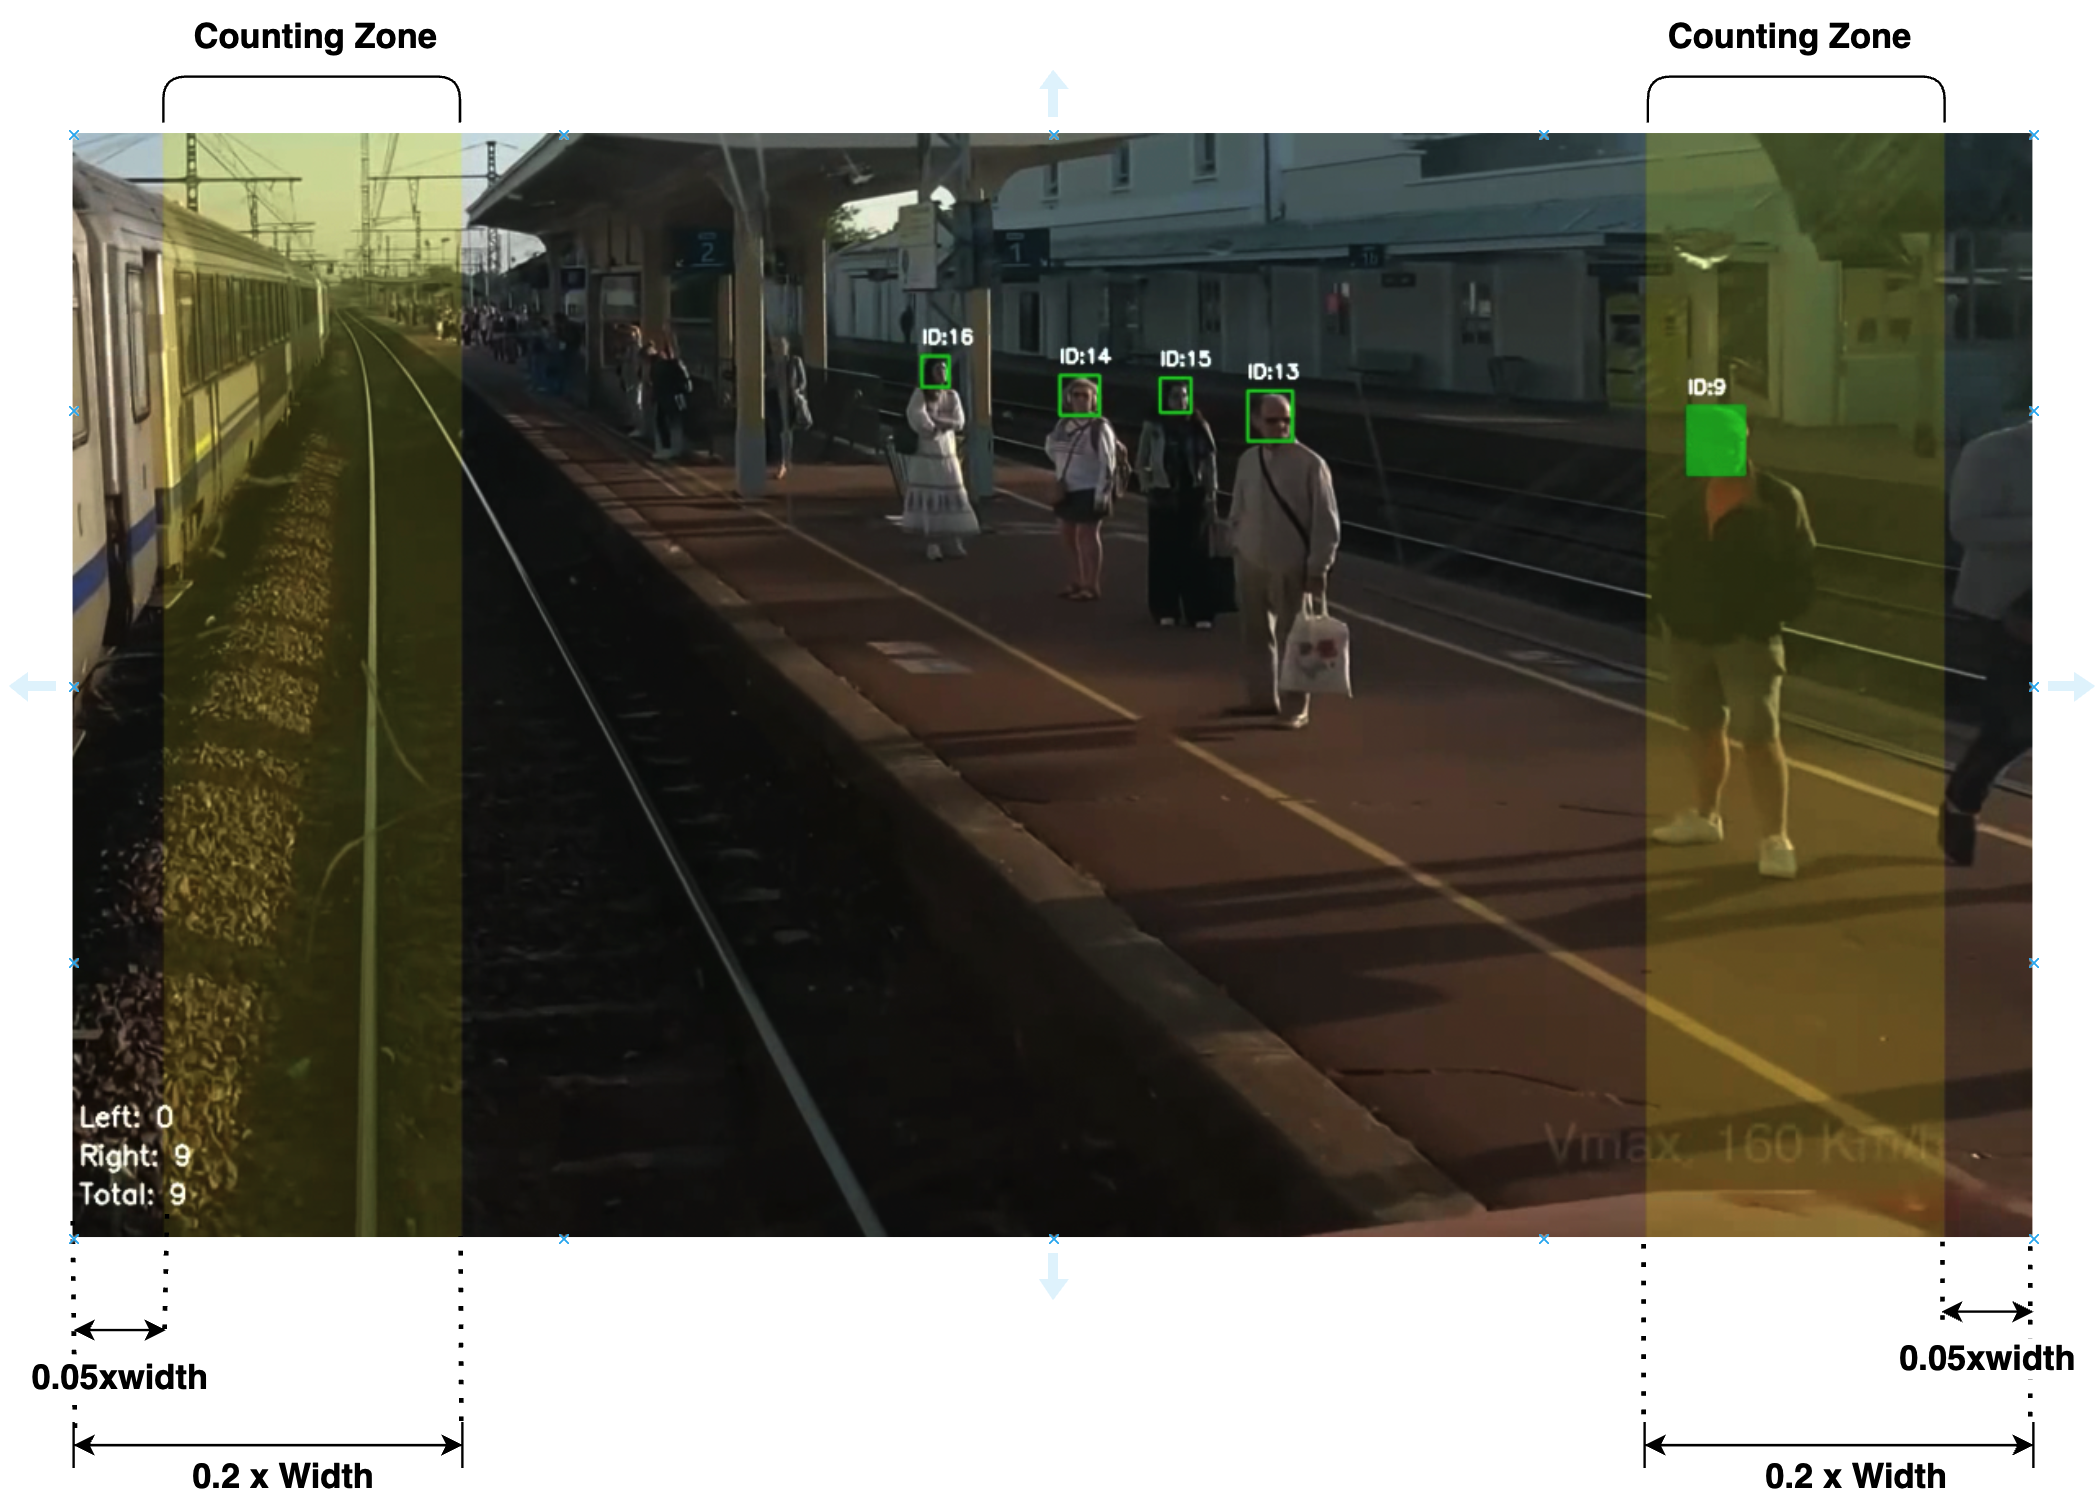
\includegraphics[width=0.49\textwidth]{pictures/VirtualCountingZone.png}
    \caption{Virtual Counting Band Illustration. The diagram shows the virtual counting zones positioned near the left and right image borders. The band is defined by start and end boundaries as proportions of image width (Start=0.05, End=0.20), creating a buffer region that tolerates brief occlusions and detection jitter. A target is counted only when it remains continuously within the band for a preset number of frames, providing robust counting under challenging conditions.}
    \label{fig:VirtualCountingZoneMethods}
\end{figure}

\textbf{Algorithm Implementation:}
\begin{enumerate}
    \item \textbf{Track State Management:} For each confirmed track, maintain state variables: consecutive\_in\_band\_frames, counted\_flag, and side\_assignment (left/right).
    \item \textbf{Band Membership Test:} Compute bounding box center $(u,v)$ and test if $u \in [\text{Start} \cdot W, \text{End} \cdot W]$ for left band or $u \in [W - \text{End} \cdot W, W - \text{Start} \cdot W]$ for right band.
    \item \textbf{Persistence Logic:} If track is in band, increment consecutive\_in\_band\_frames; otherwise reset to 0. When consecutive\_in\_band\_frames $\geq N$ and counted\_flag=False, set counted\_flag=True and increment corresponding side counter.
    \item \textbf{Deduplication:} Maintain global set of counted\_IDs to prevent double-counting across frames.
    \item \textbf{End-of-Video Compensation:} For tracks with consecutive\_in\_band\_frames $> 0$ but $< N$ at video end, apply compensation rule: if consecutive\_in\_band\_frames $\geq N/2$, count the track.
    \item \textbf{Final Aggregation:} Report left count, right count, and final count = max(left\_count, right\_count) to avoid non-platform bias.
\end{enumerate}

\subsection{Evaluation Metrics}

We evaluate our system using standard MOT metrics and counting metrics. For multi-object tracking evaluation, we adopt the CLEAR-MOT protocol \cite{bernardin2008evaluating} with metrics including Multiple Object Tracking Accuracy (MOTA), Multiple Object Tracking Precision (MOTP), Identity F1 Score (IDF1), and Identity Switches (IDSW). For identity-based evaluation, we use Identity Precision (IDP), Identity Recall (IDR), and IDF1 as defined in \cite{ristani2016performance}. 

For counting performance assessment, we employ standard regression metrics: Mean Absolute Error (MAE), Root Mean Squared Error (RMSE), Mean Absolute Percentage Error (MAPE), and Mean Error (ME) to quantify the discrepancy between predicted and ground-truth counts across all test videos.

\subsection{Camera Calibration}

To support the Phys-5D model's geometric constraints and depth estimation requirements, we perform camera calibration for each video sequence using fSpy software. Given the diverse camera setups and potential lens distortions across our dataset, we obtain multiple calibration results corresponding to different camera configurations. Based on the geometric constraint requirements in Equation~\ref{eq:geometric_constraints}, we calibrate the focal length $f$ and principal point coordinates $(c_u, c_v)$ for each video sequence. Our calibration results reveal three distinct camera configurations: (1) standard resolution cameras with focal length $f=1173.03$ pixels, (2) 4K cameras with $f=1600.3$ pixels, and (3) 2K cameras with $f=795.0$ pixels. These intrinsic parameters are essential for the Phys-5D model's 3D-to-2D projection constraints and accurate depth estimation.


\section{\uppercase{Experiment}}
\label{sec:experiment}

This section presents comprehensive experimental evaluation of our Phys-5D physics-constrained tracking system. We demonstrate the effectiveness of our 3D geometric constraints and physics-based motion modeling for railway platform crowd counting applications.

\subsection{Experimental Setup}

We evaluate our Phys-5D system using standard MOT metrics (MOTA, IDF1, IDSW) and counting metrics (MAE, RMSE, MAPE, ME) to assess tracking and counting performance.

\subsection{Training and Fine-tuning of the YOLOv11m Detector}

We adopt YOLOv11m as a balanced choice between accuracy and speed. We use a two-stage transfer learning strategy to build a head detector with strong generalization and high performance in our target domain.

\textbf{Stage 1: Pre-training} on CrowdHuman dataset to learn generic head features. The pre-training results are shown in \textbf{Fig.}~\ref{fig:yolo11mpre2results} and \textbf{Tab.}~\ref{tab:yolopre2_results}: mAP50=79.4\% and mAP50–95=54.7\%.

\begin{figure}[h]
    \centering
    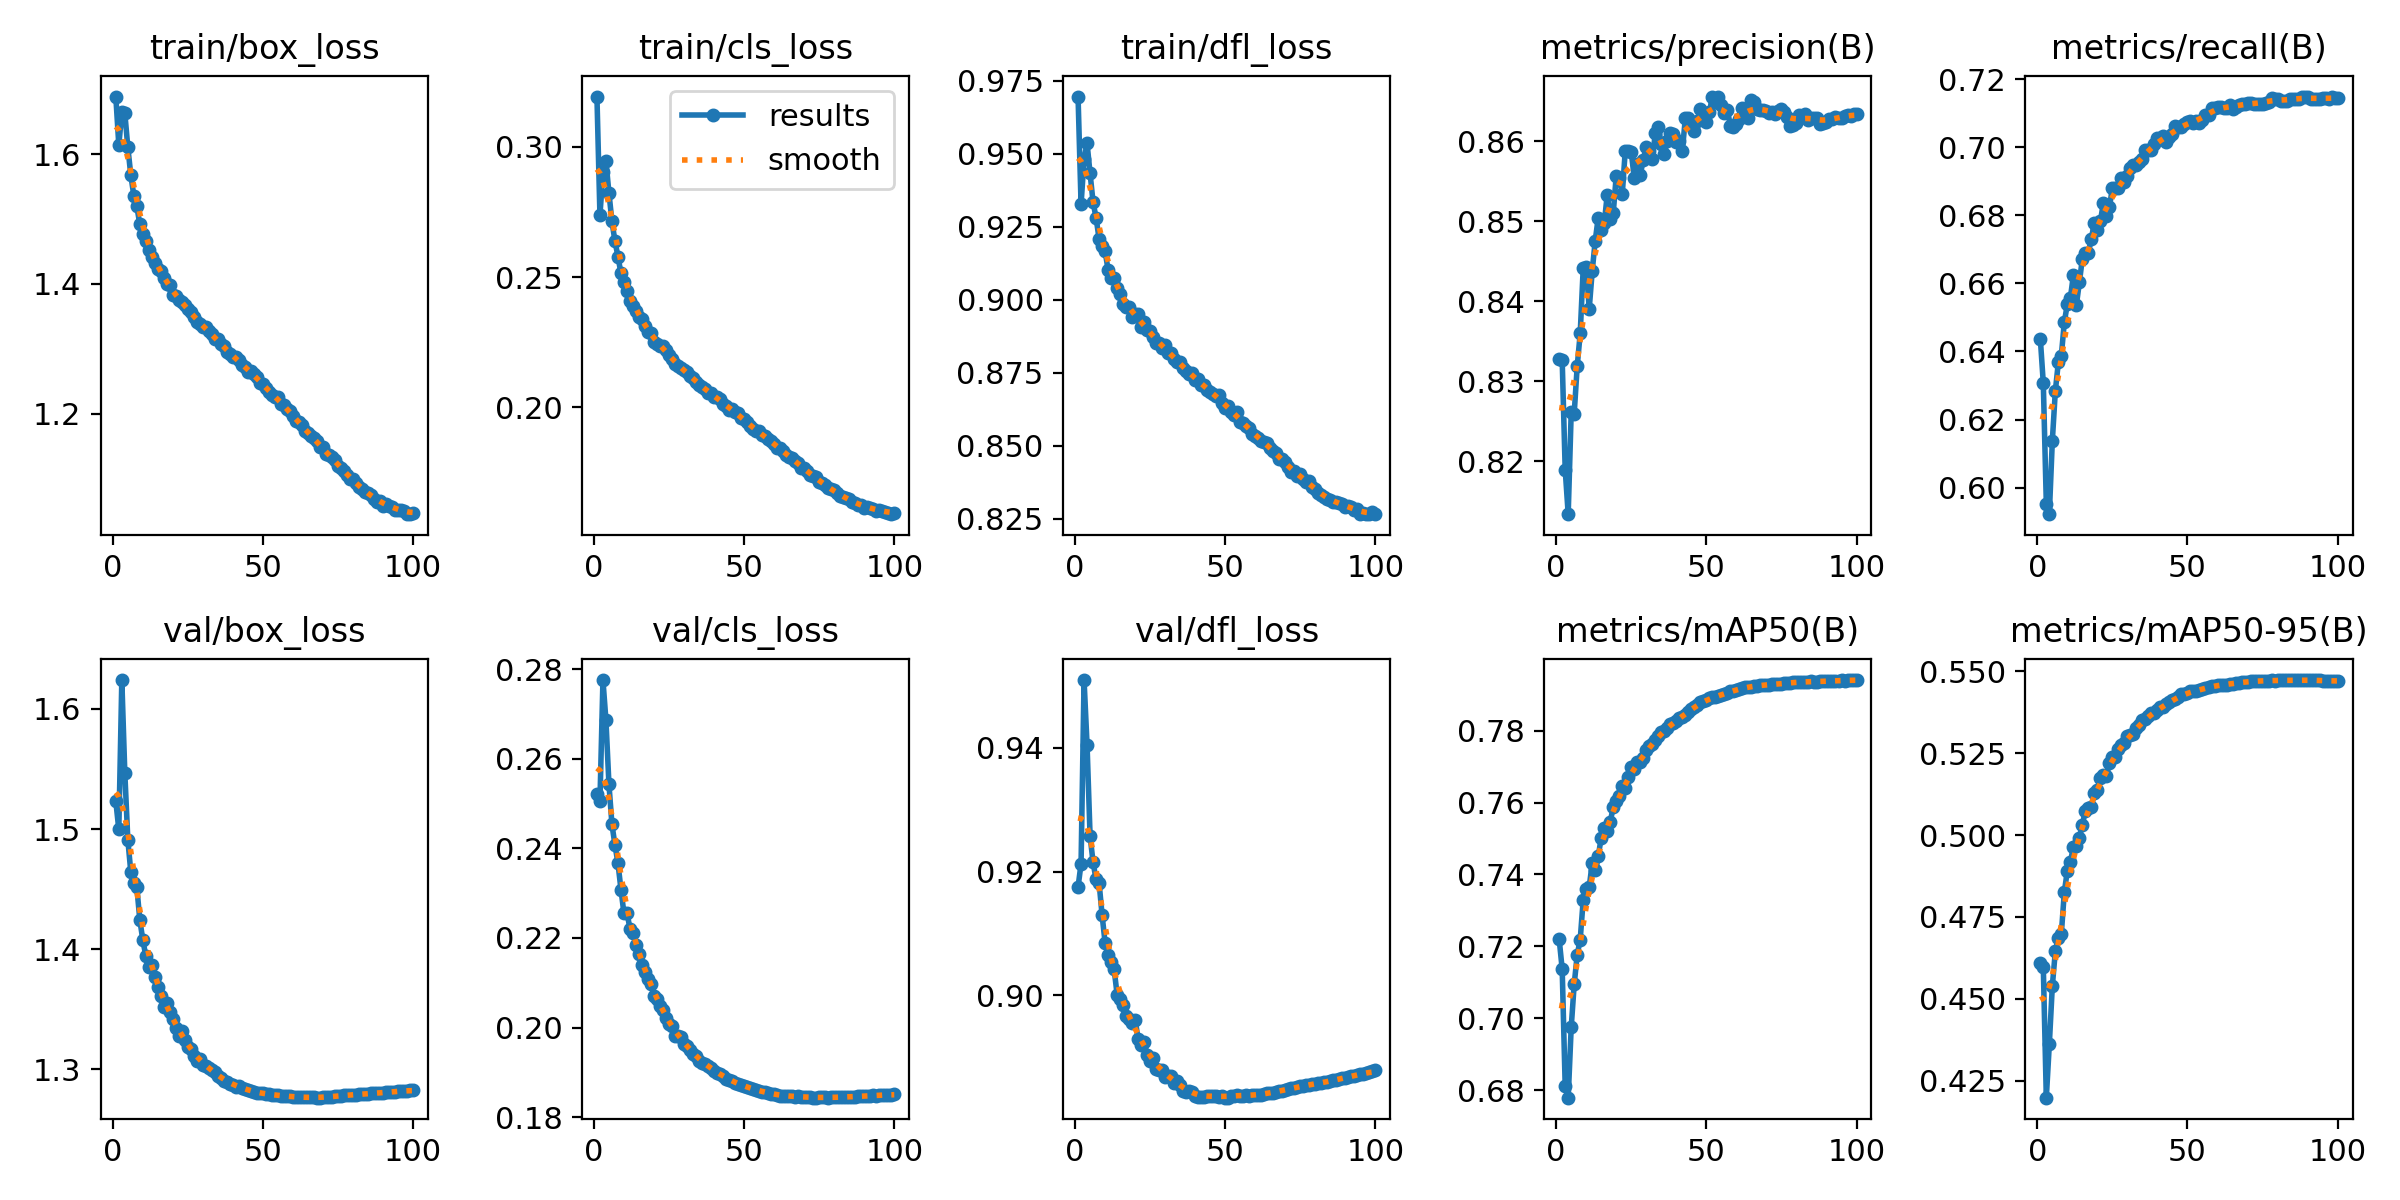
\includegraphics[width=0.48\textwidth]{pictures/yolo11mpre2results.png}
    \caption{Pre-training Results of YOLOv11m on the CrowdHuman Dataset}
    \label{fig:yolo11mpre2results}
\end{figure}

\begin{table}[h]
\centering
\resizebox{0.48\textwidth}{!}{%
\setlength{\tabcolsep}{12pt}
\renewcommand{\arraystretch}{1.3}
\begin{tabular}{|c|c|c|c|c|c|c|}
\hline
\textbf{Class} & \textbf{Images} & \textbf{Instances} & \textbf{Box(Precision)} & \textbf{Recall} & \textbf{mAP50} & \textbf{mAP50–95} \\
\hline
all & 4370 & 98568 & 0.862 & 0.715 & 0.794 & 0.547 \\
\hline
\end{tabular}%
}
\caption{Pre-training Performance of YOLOv11m on the CrowdHuman Dataset}
\label{tab:yolopre2_results}
\end{table}

\textbf{Stage 2: Fine-tuning} with backbone=10 frozen on railway platform head images achieves mAP50=98.0\% (+18.6 points) and mAP50–95=81.6\% (+26.9 points).

\begin{figure}[h]
    \centering
    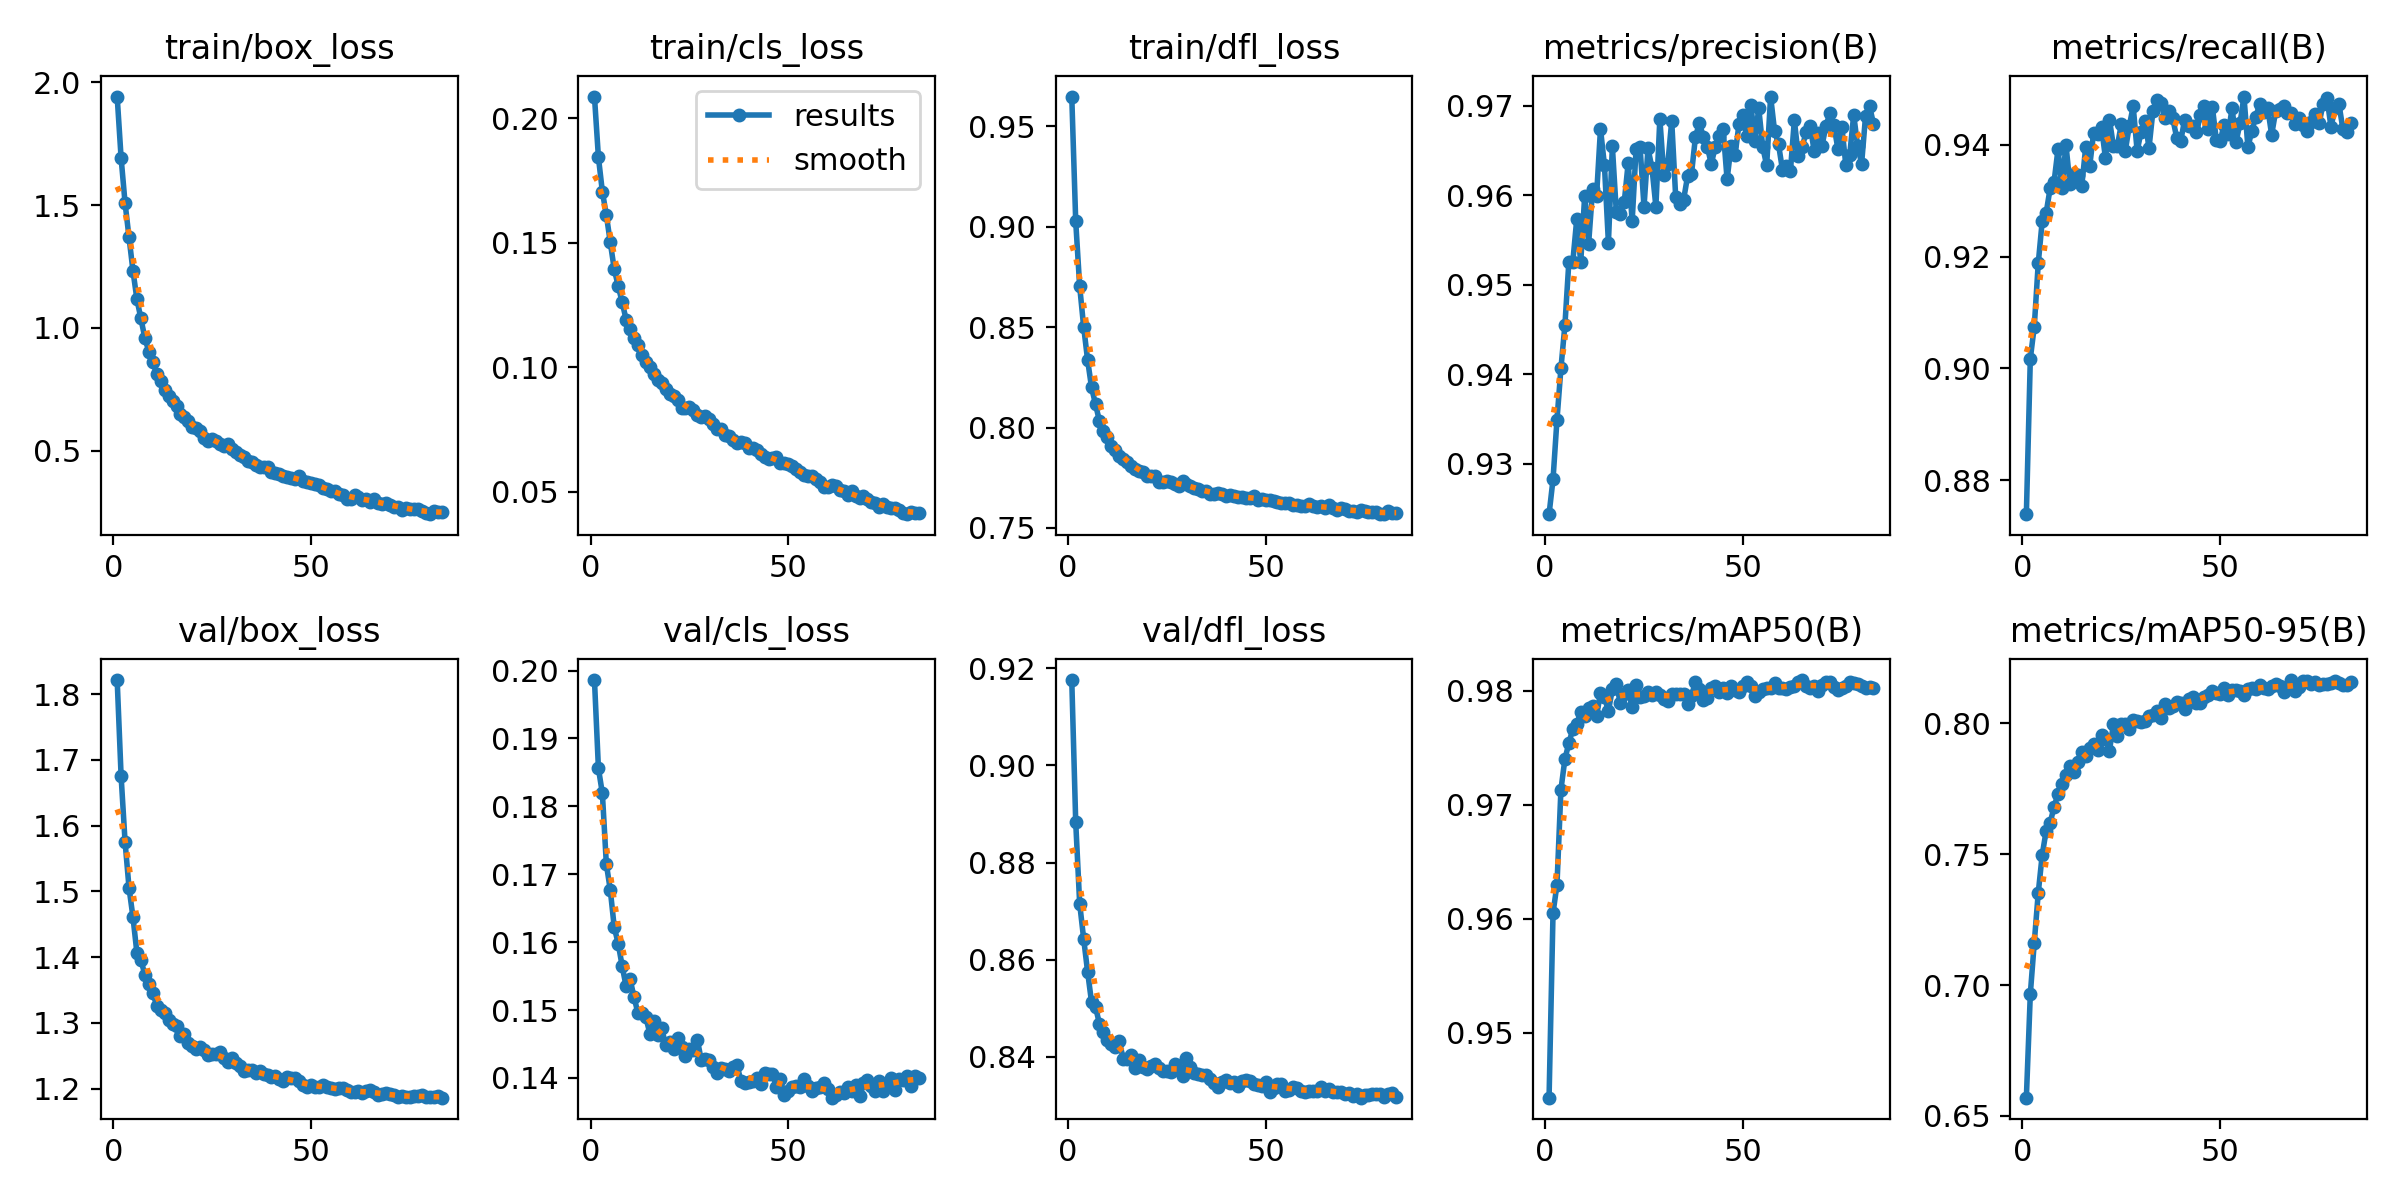
\includegraphics[width=0.48\textwidth]{pictures/yolofreez10_ResultsSummary.png}
    \caption{Fine-tuning Results of YOLOv11m on the Custom Head Dataset}
    \label{fig:yolo11mfinetuneresults}
\end{figure}

\begin{table}[h]
\centering
\resizebox{0.48\textwidth}{!}{%
\setlength{\tabcolsep}{12pt}
\renewcommand{\arraystretch}{1.3}
\begin{tabular}{|c|c|c|c|c|c|c|}
\hline
\textbf{Class} & \textbf{Images} & \textbf{Instances} & \textbf{Box(P)} & \textbf{R} & \textbf{mAP50} & \textbf{mAP50–95} \\
\hline
all & 600 & 4779 & 0.965 & 0.946 & 0.980 & 0.816 \\
\hline
\end{tabular}%
}
\caption{Fine-tuning Performance of YOLOv11m freeze=10 on the Labeled Head Dataset}
\label{tab:yolofreeze10_results}
\end{table}

\subsection{EfficientNet-B0 ReID Model Experimental Setup and Results}

We adopt EfficientNet-B0 as the ReID backbone to balance efficiency and accuracy. The ReID training dataset consists of 7 video sequences with 238 tracked identities from our MOT-RPCH dataset.

\subsubsection{ReID Input Size Ablation Study}

To determine the optimal input resolution for our ReID model, we conduct a comprehensive ablation study comparing different input sizes under identical training settings. This study evaluates the speed-accuracy trade-offs across multiple resolutions.

\begin{figure}[h]
    \centering
    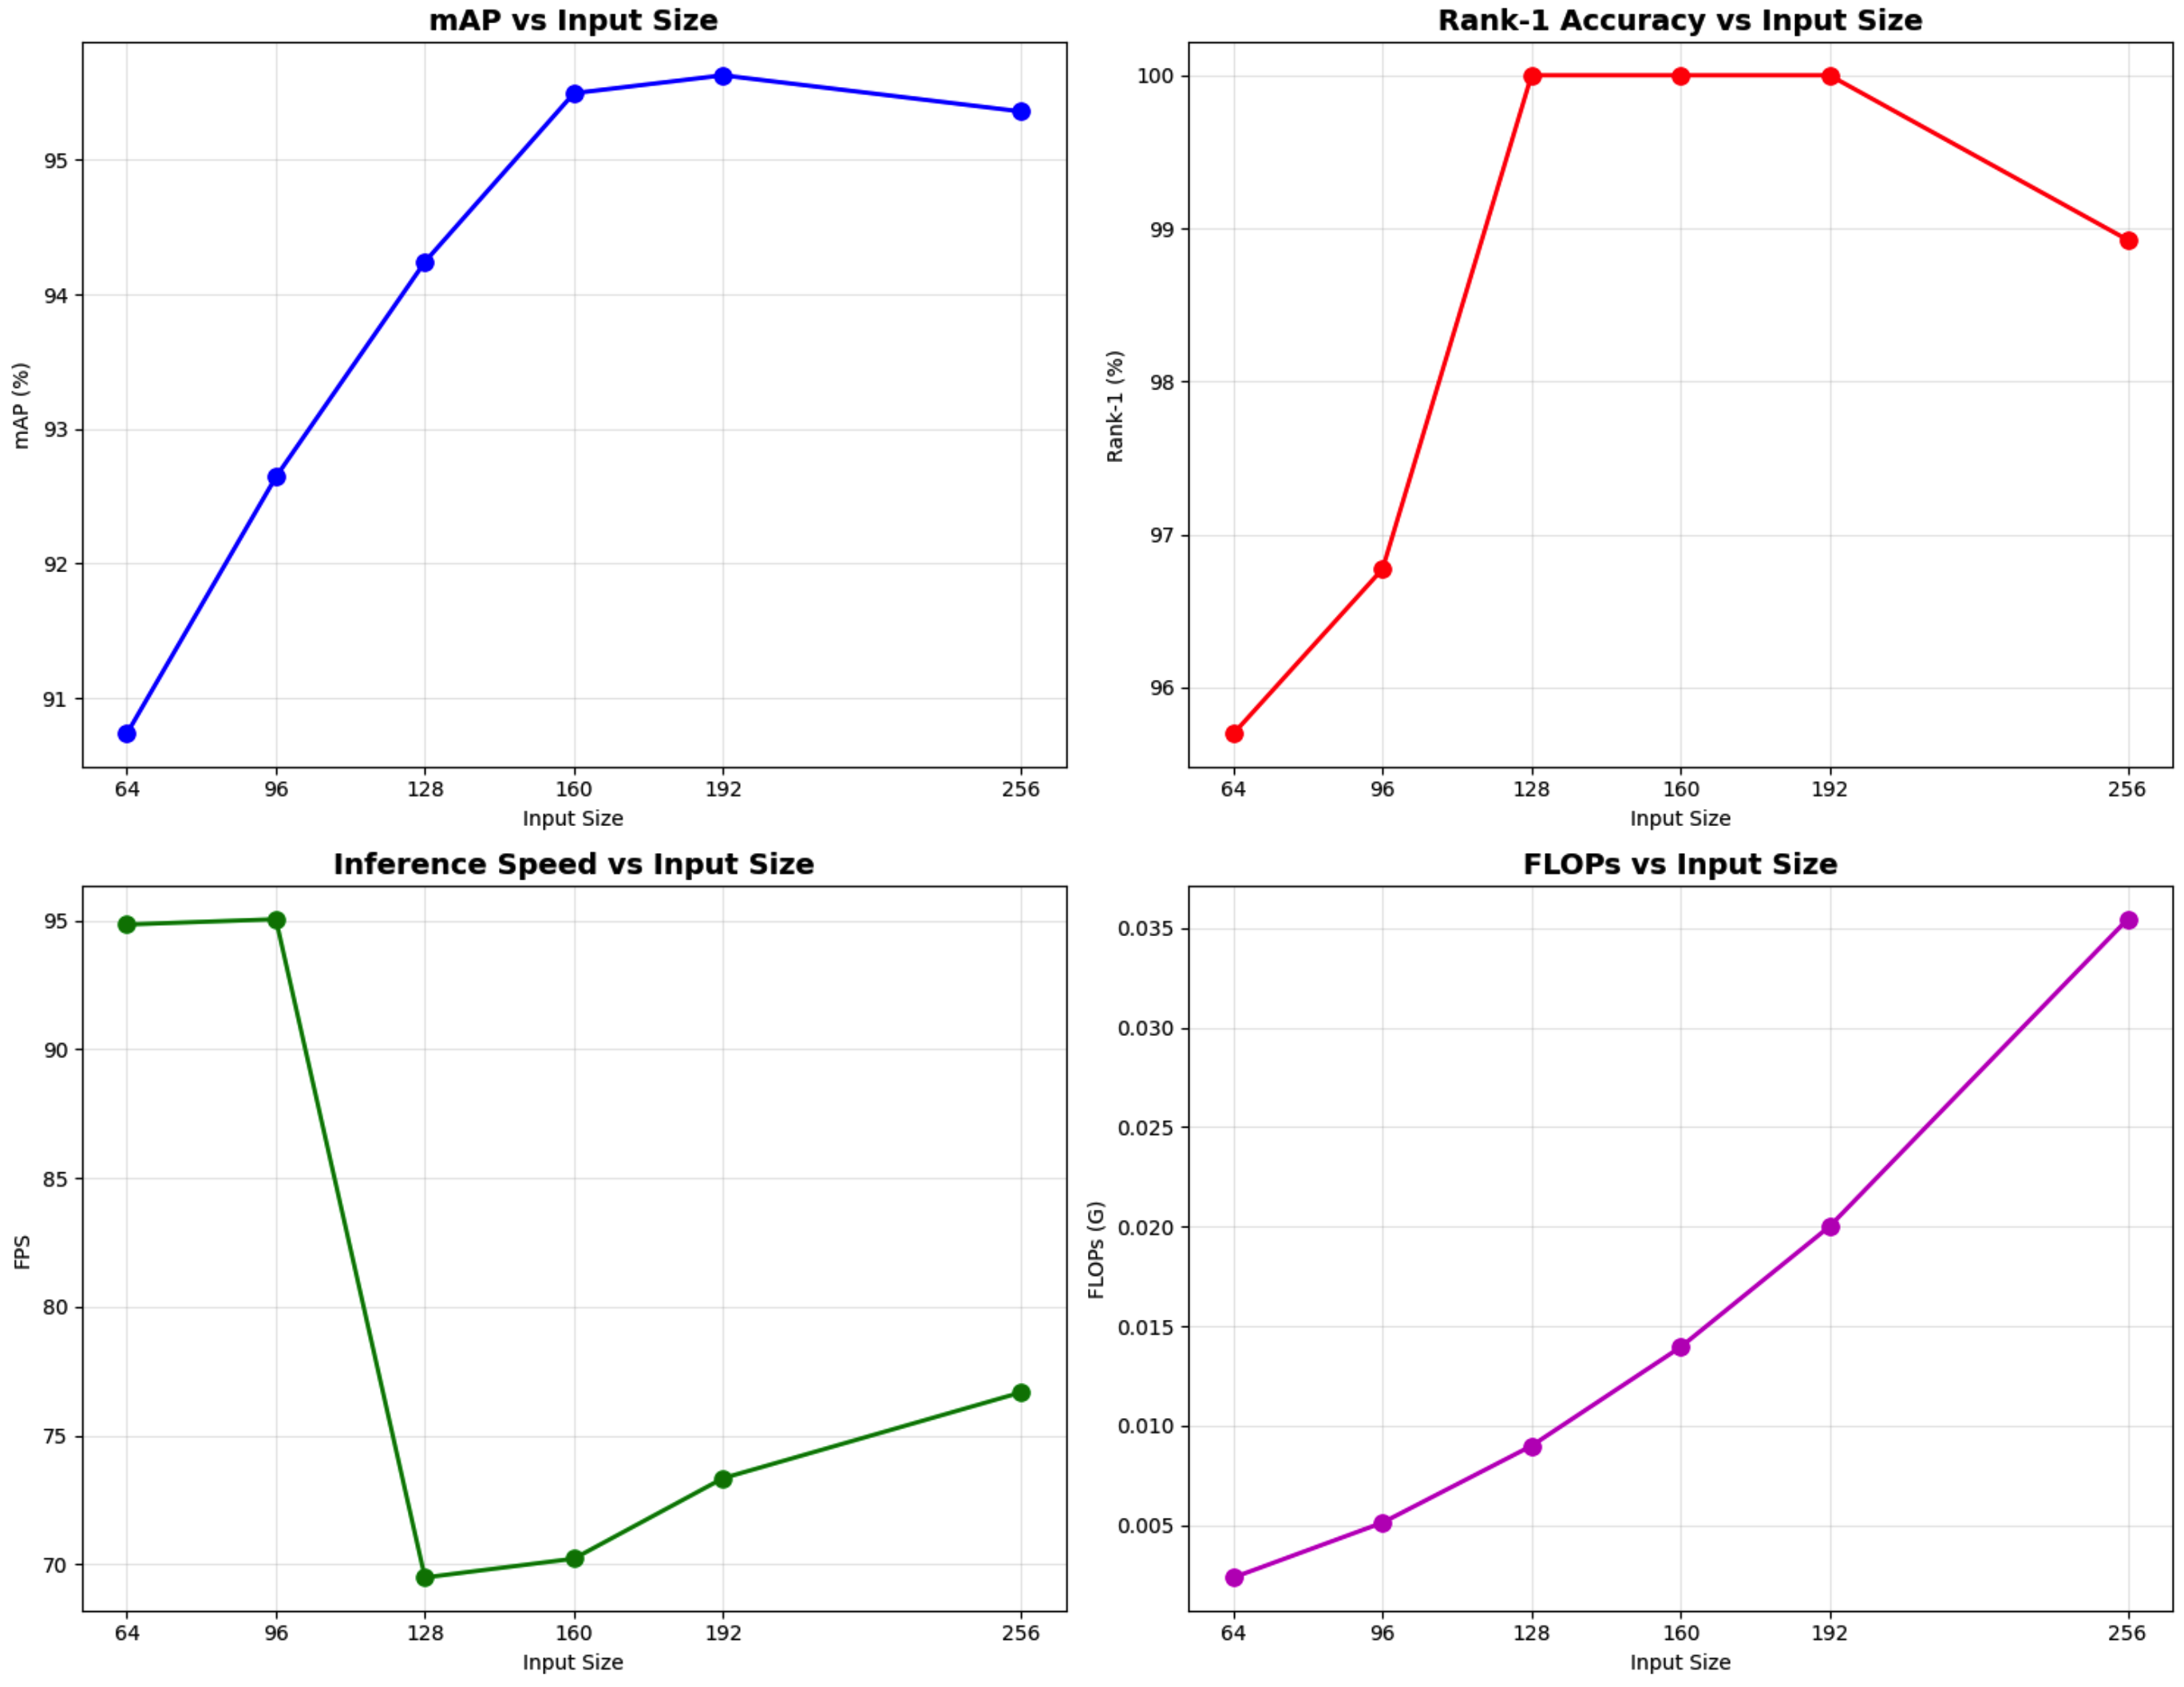
\includegraphics[width=0.48\textwidth]{pictures/ReIDInputsizeAblationexperiment.png}
    \caption{ReID Input Size Ablation Experiment Results}
    \label{fig:ReIDInputsizeAblationexperiment}
\end{figure}

As shown in \textbf{Fig.}~\ref{fig:ReIDInputsizeAblationexperiment} and \textbf{Tab.}~\ref{tab:ReIDablationexperiment}, we evaluate six different input resolutions from 64×64 to 256×256 pixels. The results demonstrate clear performance improvements with increasing resolution, but with diminishing returns and increased computational cost.

\begin{table}[h]
    \centering
    \resizebox{0.45\textwidth}{!}{%
    \renewcommand{\arraystretch}{1.3}
    \begin{tabular}{|c|c|c|c|c|c|c|}
    \hline
        \textbf{Input Size (pix)} & \textbf{mAP (\%)} & \textbf{Rank-1 (\%)} & \textbf{FPS} & \textbf{FLOPs (G)} & \textbf{Parameter quantity} & \textbf{Marginal benefits} \\ \hline
        64x64 & 90.74 & 95.7 & 94.8 & 0.002 & 206240 & 0 \\
        96x96 & 92.64 & 96.77 & 95 & 0.005 & 206240 & +1.90 mAP \\
        128x128 & 94.24 & 100 & 69.5 & 0.009 & 206240 & +1.60 mAP \\
        160x160 & 95.49 & 100 & 70.2 & 0.014 & 206240 & +1.25 mAP \\
        192x192 & 95.63 & 100 & 73.3 & 0.02 & 206240 & +0.14 mAP \\
        256x256 & 95.36 & 98.92 & 76.7 & 0.035 & 206240 & –0.27 mAP \\ \hline
    \end{tabular}%
    }
    \caption{ReID Ablation Experiment Results}
    \label{tab:ReIDablationexperiment}
\end{table}

\textbf{Key Findings:}
\begin{itemize}
    \item \textbf{Performance Improvement:} Increasing resolution from 64×64 to 128×128 improves mAP by 3.50\% and Rank-1 by 4.30\%, representing significant accuracy gains.
    \item \textbf{Diminishing Returns:} Beyond 128×128, performance improvements become marginal (+1.25 mAP for 160×160, +0.14 mAP for 192×192).
    \item \textbf{Computational Efficiency:} 128×128 provides the best balance, achieving Rank-1=100\% with only 0.009 GFLOPs and 69.5 FPS inference on NVIDIA T4 GPU.
    \item \textbf{Performance Degradation:} 256×256 shows slight performance degradation (mAP drops by 0.27\%) while requiring significantly more computation.
\end{itemize}

Based on this comprehensive analysis, we select 128×128 as our final ReID input resolution, achieving optimal performance with Rank-1=100\%, mAP=94.24\%, and efficient real-time inference capability.

\subsection{Three Models Comparison}

To assess the role of different tracking approaches in MOT, we conduct a comprehensive comparison of three distinct tracking models. We evaluate: (i) the 8D constant-velocity baseline (CV-8D) with standard DeepSORT parameters, (ii) a 12D constant-acceleration model (CA-12D) with adjusted noise modeling for higher dimensionality, and (iii) a 5D physics-constrained model (Phys-5D) with specialized camera calibration and physics-based constraints.

\subsubsection{Comparative Analysis of Three Kalman State-Space Model Configurations}

We evaluate three distinct tracking models, each optimized with its own best-performing configuration. \textbf{Tab.}~\ref{tab:3modelsCountingComparisonResults} compares their counting performance under these optimized settings.

\begin{table}[h]
    \centering
    \resizebox{0.48\textwidth}{!}{%
    \small
    \begin{tabular}{|c|c|c|c|c|}
    \hline
        \textbf{Model} & \textbf{MAE } & \textbf{RMSE} & \textbf{MAPE(\%)} & \textbf{ME } \\ \hline
        \textbf{CV-8D} & 3.4 & 6.1514 & 14.592 & 1.4  \\ 
        \textbf{CA-12D} & 2.4 & 4.5837 & 6.99 & 0.7  \\ 
        \textbf{Phys-5D} & 0.75 & 1.3229 & 2.236 & -0.25 \\ \hline
    \end{tabular}%
    }
    \caption{Counting Performance Comparison of the Three Models}
    \label{tab:3modelsCountingComparisonResults}
\end{table}

\textbf{Results Summary:} The three models show distinct performance characteristics. CV-8D achieves baseline performance with MAPE=14.59\%, CA-12D reduces counting error to MAPE=6.99\%, and Phys-5D achieves the best performance with MAPE=2.24\%.

\subsection{Phys-5D Model Performance}

\subsubsection{Overall Tracking Results}
Our Phys-5D model achieves superior performance with the following key metrics:

\begin{table}[h]
\centering
\resizebox{0.48\textwidth}{!}{%
\small
\renewcommand{\arraystretch}{1.3}
\begin{tabular}{|l|c|c|c|c|c|c|}
\hline
\textbf{Metric} & \textbf{MOTA} & \textbf{IDF1} & \textbf{IDSW} & \textbf{Precision} & \textbf{Recall} & \textbf{FAF} \\
\hline
Phys-5D & 67.21\% & 76.29\% & 24.8 & 89.06\% & 77.45\% & 0.32 \\
\hline
\end{tabular}%
}
\caption{Phys-5D Model Performance}
\label{tab:Phys5D_Performance}
\end{table}

The Phys-5D model demonstrates excellent tracking stability with low identity switches (24.8 average) and high precision (89.06\%), indicating effective identity preservation under challenging railway platform conditions.

\subsubsection{Counting Performance}
Our Phys-5D system achieves state-of-the-art counting accuracy:

\begin{table}[h]
\centering
\resizebox{0.48\textwidth}{!}{%
\small
\renewcommand{\arraystretch}{1.3}
\begin{tabular}{|l|c|c|c|c|}
\hline
\textbf{Metric} & \textbf{MAE} & \textbf{RMSE} & \textbf{MAPE (\%)} & \textbf{ME} \\
\hline
Phys-5D & 0.75 & 1.32 & 2.24 & -0.25 \\
\hline
\end{tabular}%
}
\caption{Phys-5D Counting Performance}
\label{tab:Phys5D_Counting}
\end{table}

The Phys-5D model achieves exceptional counting accuracy with MAPE=2.24\%, demonstrating the effectiveness of physics-constrained 3D tracking for crowd counting applications.

\subsection{Phys-5D Detailed Results}

\subsubsection{Per-Video Analysis}
We analyze Phys-5D performance across different video characteristics:

\begin{table}[h]
\centering
\resizebox{0.48\textwidth}{!}{%
\small
\renewcommand{\arraystretch}{1.3}
\begin{tabular}{|l|c|c|c|c|c|c|c|c|c|c|}
\hline
\textbf{Metric} & \textbf{MOTA} & \textbf{MOTP} & \textbf{IDF1} & \textbf{IDP} & \textbf{IDR} & \textbf{IDSW} & \textbf{Precision} & \textbf{Recall} & \textbf{FAF} & \textbf{MAPE} \\
\hline
\textbf{Average} & 67.21\% & 17.41 & 76.29\% & 82.23\% & 71.51\% & 24.8 & 89.06\% & 77.45\% & 0.32 & 2.24\% \\
\hline
\end{tabular}%
}
\caption{Phys-5D Average Performance Results (Detailed per-video results are provided in Appendix)}
\label{tab:Phys5D_Average_Results}
\end{table}

Table \ref{tab:Phys5D_Average_Results} summarizes the average performance metrics of the YOLOv11 + DeepSORT tracking system on the Phys-5D dataset across 20 test videos. Overall, the model achieved an average MOTA of 67.21\% and an IDF1 score of 76.29\%, indicating a good balance between detection accuracy and identity consistency. 
The mean precision and recall were 89.06\% and 77.45\%, respectively, with an average MAPE of 2.24\% for bidirectional counting, demonstrating reliable counting accuracy. Most sequences exhibited stable tracking performance, with relatively low identity switches (mean = 24.8) and consistent ID precision across diverse video conditions. Detailed per-video results are provided in the Appendix.

\subsection{Ablation Studies}

To validate the effectiveness of individual components in our Phys-5D system, we conduct comprehensive ablation studies on the detector, ReID model, and counting method.

\subsubsection{YOLOv11m Detector Ablation Study}
We design an ablation study to examine the fine-tuned detector's sensitivity to hyperparameters. We vary three key hyperparameters—input size, confidence threshold, and IoU threshold—yielding 64 combinations. Through comprehensive evaluation across all parameter combinations, we identify the optimal configuration that achieves the best balance between detection accuracy and inference speed.

\begin{table}[h]
    \centering
    \resizebox{0.48\textwidth}{!}{%
    \small
    \renewcommand{\arraystretch}{1.3}
    \begin{tabular}{|c|c|c|c|c|c|c|c|}
    \hline
        \textbf{Conf} & \textbf{IoU} & \textbf{Imgsz} & \textbf{mAP50} & \textbf{mAP50-95} & \textbf{Precision} & \textbf{Recall} & \textbf{Inference\_Time(ms)} \\
    \hline
        0.3 & 0.3 & 736 & 0.9224 & 0.6871 & 0.9193 & 0.8707 & 16.86 \\
    \hline
    \end{tabular}%
    }
    \caption{Optimal YOLOv11m Detector Configuration (Complete ablation results are provided in Appendix)}
    \label{tab:YOLO11m_Optimal_Config}
\end{table}

The optimal configuration achieves mAP50=92.24\% and mAP50-95=68.71\% with precision=91.93\% and recall=87.07\%, while maintaining reasonable inference time of 16.86ms. This configuration demonstrates the effectiveness of moderate confidence and IoU thresholds combined with 736-pixel input resolution for railway platform head detection. The complete ablation study results across all 64 parameter combinations are provided in the Appendix for detailed analysis.


\subsubsection{Ablation Study of the Counting Method}

We evaluate the proposed Virtual Counting Band and its hyperparameters. The band introduces nonzero width and a persistence criterion to overcome line-crossing brittleness under jitter and occlusion. We focus on the start and end positions.

\begin{figure}[h]
    \centering
    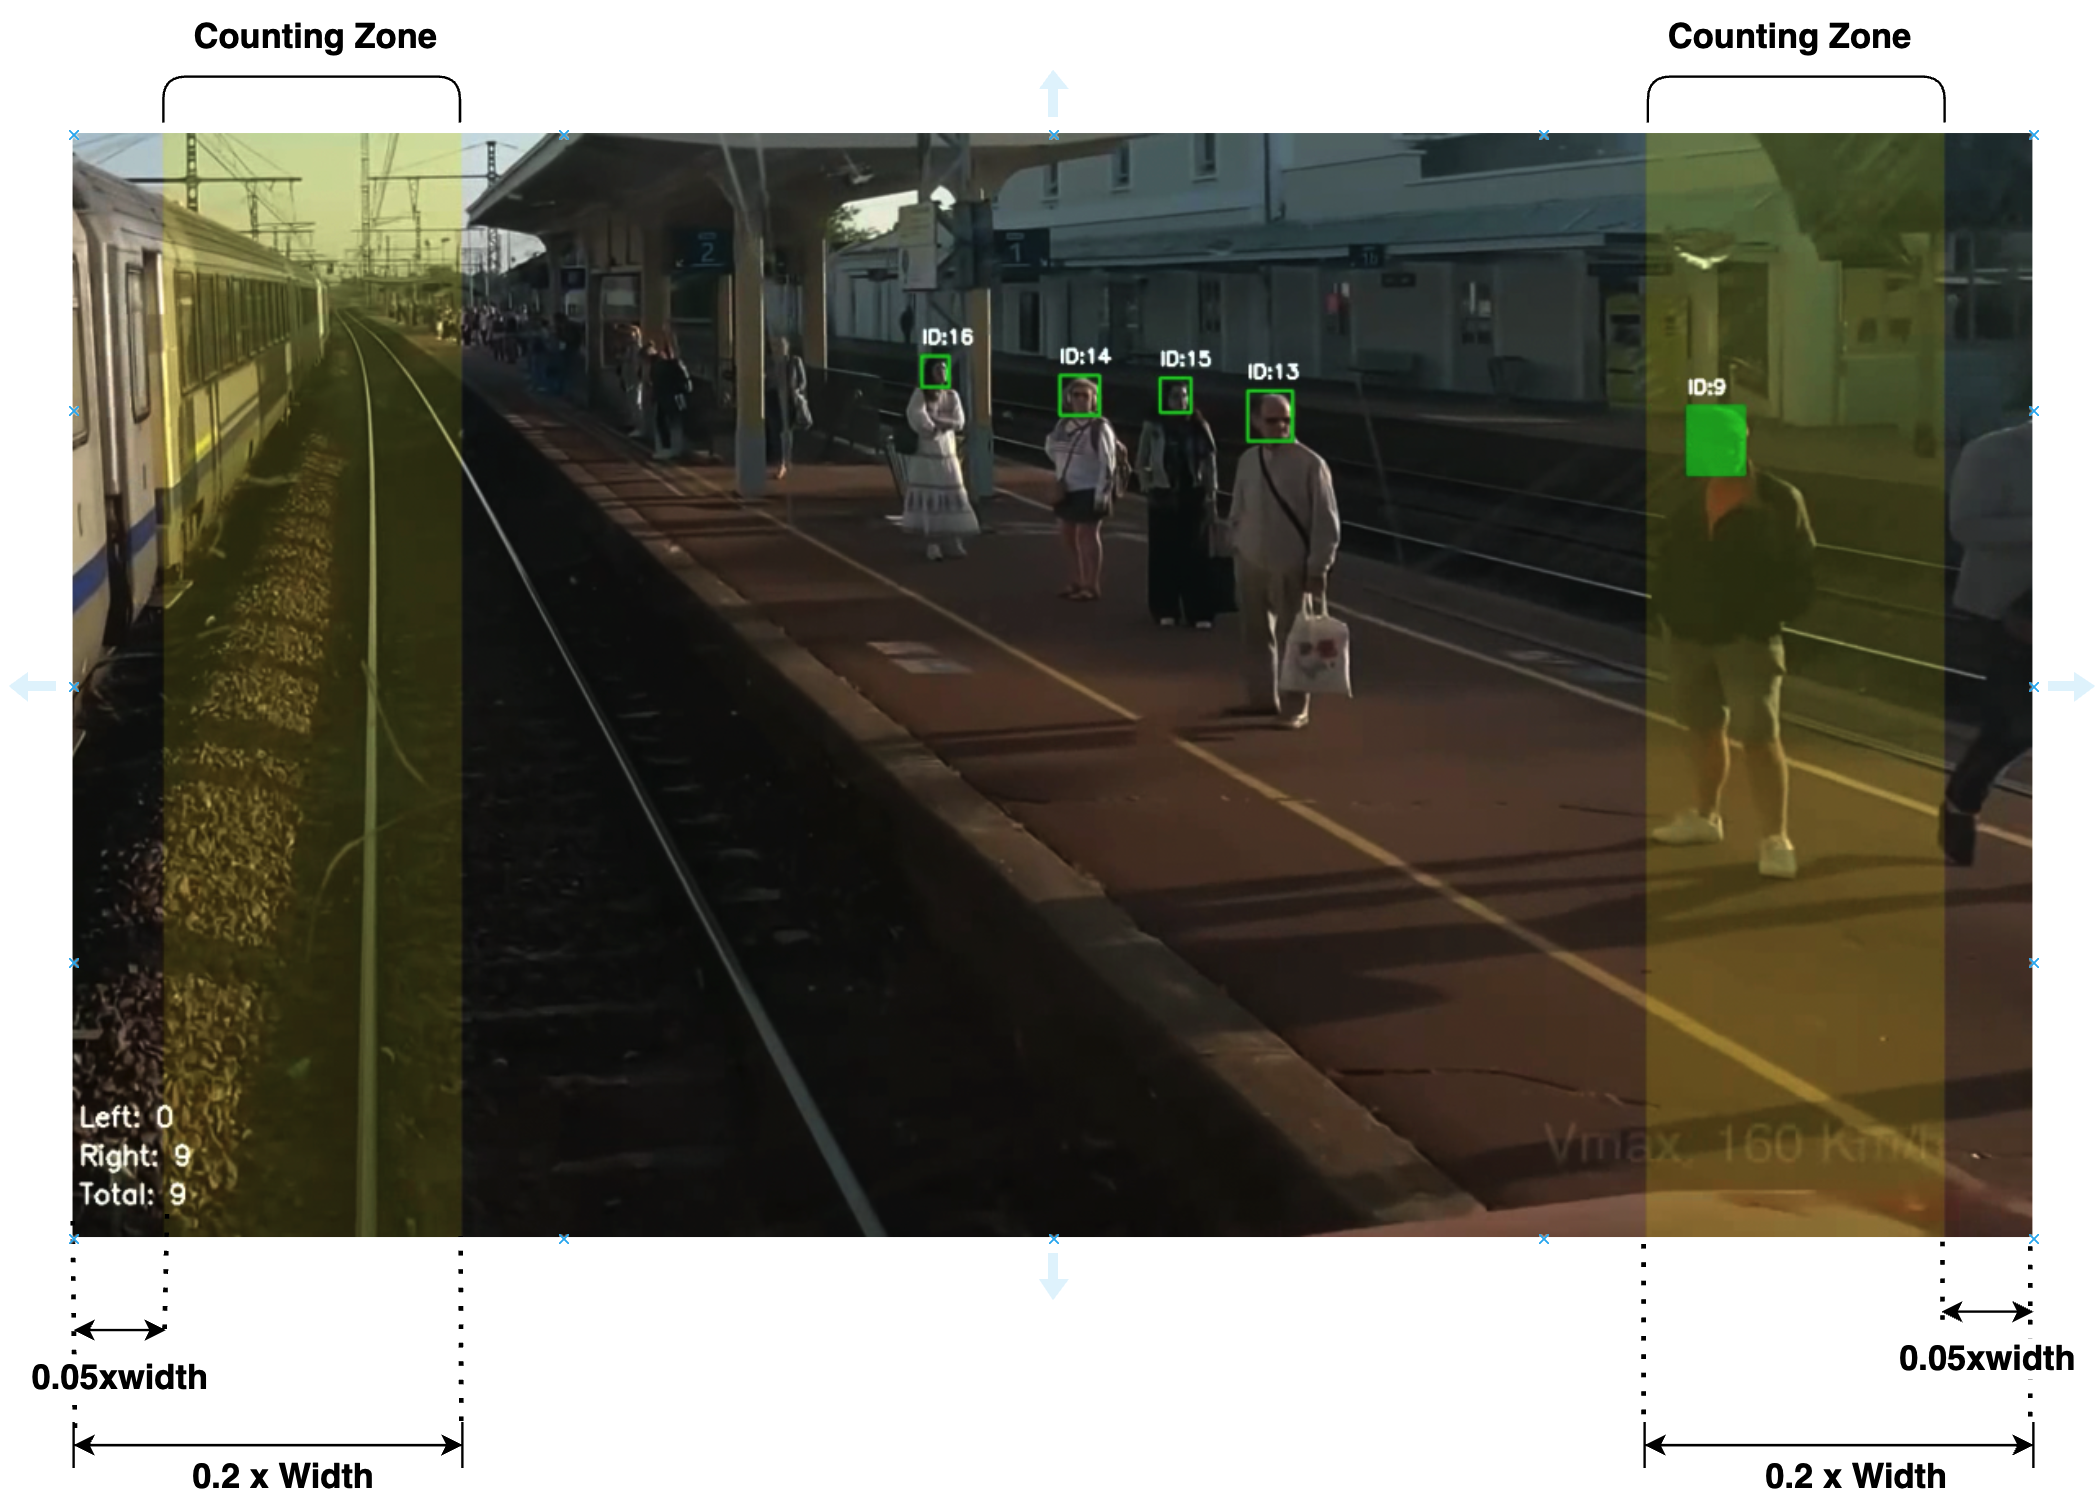
\includegraphics[width=0.48\textwidth]{pictures/VirtualCountingZone.png}
    \caption{Schematic Diagram of the Virtual Counting Zone}
    \label{fig:VirtualCountingZone}
\end{figure}

Through comprehensive evaluation of virtual counting band configurations, we systematically analyze the impact of start and end positions on counting performance. Our analysis reveals that the optimal configuration achieves exceptional counting accuracy with minimal systematic bias.

\begin{table}[h]
    \centering
    \resizebox{0.48\textwidth}{!}{%
    \small
    \renewcommand{\arraystretch}{1.3}
    \begin{tabular}{|c|c|c|c|c|c|}
    \hline
        \textbf{Start} & \textbf{End} & \textbf{MAE} & \textbf{RMSE} & \textbf{MAPE(\%)} & \textbf{ME} \\
    \hline
        0.05 & 0.20 & 0.90 & 1.38 & 2.97 & -0.20 \\
    \hline
    \end{tabular}%
    }
    \caption{Optimal Virtual Counting Band Configuration (Complete ablation results are provided in Appendix)}
    \label{tab:Optimal_Counting_Band}
\end{table}

The optimal configuration (Start=0.05, End=0.20) achieves exceptional counting performance with MAE=0.90, RMSE=1.38, MAPE=2.97\%, and ME=-0.20, indicating near-unbiased counting with minimal variance. This configuration demonstrates the effectiveness of a moderate-width counting band positioned near the image borders, providing robust counting under challenging conditions while maintaining high accuracy. The complete ablation study results across all parameter combinations are provided in the Appendix for detailed analysis.

\textbf{Tab.}~\ref{tab:ComparisonofAverage} further contrasts average metrics for line vs band: the band dramatically outperforms the line across MAE, RMSE, MAPE, and ME, demonstrating superior robustness and accuracy.

\begin{table}[h]
    \centering
    \resizebox{0.45\textwidth}{!}{%
    \begin{tabular}{|p{2.8cm}|c|c|c|c|}
    \hline
        \textbf{Method} & \textbf{MAE} & \textbf{RMSE} & \textbf{MAPE(\%)} & \textbf{ME} \\ \hline
        \raggedright Average metrics of line-crossing counting & 31.28 & 43.66 & 93.43 & -31.28 \\ \hline
        \raggedright Average counting metrics of counting zones & 3.13 & 4.75 & 10.87 & 0.81 \\ \hline
    \end{tabular}%
    }
    \caption{Comparison of Average Counting Metrics Lines vs. Zones}
    \label{tab:ComparisonofAverage}
\end{table}



\subsection{Summary}

Our comprehensive evaluation of the Phys-5D system demonstrates:

\textbf{Superior Counting Accuracy:} Phys-5D achieves MAPE=2.24\%, representing a significant improvement over baseline methods (CV-8D: 14.59\%, CA-12D: 6.99\%) and demonstrating the effectiveness of physics-constrained 3D tracking.

\textbf{Robust Tracking Performance:} The system maintains high tracking accuracy (MOTA=67.21\%, IDF1=76.29\%) with low identity switches (24.8 average), indicating effective identity preservation under challenging conditions.

\textbf{Component Effectiveness:} Ablation studies confirm the importance of YOLOv11m detector optimization, EfficientNet-B0 ReID backbone selection, and virtual counting band design for overall system performance.

\textbf{Real-time Capability:} The complete system processes at 29.7 FPS on NVIDIA T4 GPU, meeting practical deployment requirements for railway platform monitoring.

These results establish Phys-5D as a state-of-the-art solution for railway platform crowd counting, combining superior accuracy with real-time performance through physics-informed 3D tracking.


\section{\uppercase{Conclusion}}
\label{sec:conclusion}
This section concludes our work on physics-constrained 3D tracking for railway platform crowd counting, synthesizing key findings, theoretical implications, and future research directions.

\subsection{Research Contributions and Key Findings}

Our comprehensive evaluation demonstrates the effectiveness of physics-informed machine learning in computer vision applications. The experimental results reveal a clear performance hierarchy across the three motion models, with Phys-5D achieving superior counting accuracy (MAPE=2.24\%) compared to baseline methods (CV-8D: 14.59\%, CA-12D: 6.99\%), while maintaining robust tracking performance (MOTA=67.21\%, IDF1=76.29\%) with low identity switches (24.8 average).

\textbf{Key Theoretical Contributions:}
\begin{itemize}
    \item \textbf{Physics-Constrained 3D Tracking:} By lifting estimation from 2D image plane to 3D physical space through pinhole geometry constraints, we achieve superior robustness and accuracy compared to traditional 2D tracking approaches.
    \item \textbf{Component Synergy:} The detect–track–count pipeline demonstrates how carefully designed components (YOLOv11m detection, EfficientNet-B0 ReID, Phys-5D tracking, virtual counting band) work together for system-level excellence.
    \item \textbf{Application-Oriented Evaluation:} Our focus on counting accuracy metrics (MAE, RMSE, MAPE) rather than traditional MOT metrics reveals the true performance characteristics for crowd counting applications, where tracking serves as a means to achieve accurate counting.
\end{itemize}

\textbf{Critical Insight:} The results demonstrate that incorporating domain knowledge through physics constraints is far more effective than merely increasing kinematic model complexity. While CA-12D and Phys-5D achieve similar MOTA scores (67.54\% vs 67.21\%), Phys-5D's superior identity consistency (24.8 vs 39.15 ID switches) directly translates to superior counting accuracy. This highlights that for cumulative tasks like counting, trajectory stability and persistent identity are more important than single-frame localization accuracy.

\subsection{Practical Value and Deployment Readiness}

Our Phys-5D system achieves deployment-ready accuracy with 2.24\% counting error and real-time processing at 29.7 FPS on NVIDIA T4 GPU. The precise crowd counting capability provides multi-dimensional insights for railway station management:

\textbf{Real-time Safety and Density Management:} Accurate passenger counts enable real-time density monitoring with automatic alerts to prevent overcrowding and ensure passenger safety. The system can identify peak density periods and trigger crowd control measures.

\textbf{Operational Efficiency and Scheduling:} Historical and real-time counting data supports intelligent scheduling decisions, allowing operators to adjust train frequencies based on actual passenger demand rather than estimates. This leads to optimized resource allocation and reduced operational costs.

\textbf{Capacity Planning and Infrastructure Development:} Long-term counting data reveals usage patterns that inform station capacity planning, platform design improvements, and infrastructure investment decisions. Understanding peak usage times helps optimize station layout and facility placement.

\textbf{Urban Mobility and Transportation Analytics:} Station-level passenger counting data provides insights into local transportation patterns, commuting behaviors, and urban mobility trends. This information supports broader transportation planning and policy decisions at the city level.

\textbf{Economic Impact Assessment:} Accurate passenger counts enable precise measurement of station utilization, supporting cost-benefit analyses for service improvements and infrastructure investments.

\textbf{Emergency Preparedness:} Reliable counting data is crucial for evacuation planning during emergencies, ensuring appropriate emergency response resources are allocated based on actual passenger numbers.

\subsection{Theoretical Implications and Broader Impact}

Our work provides compelling evidence for Physics-Informed Machine Learning (PIML) in computer vision. While recent trends favor larger, purely data-driven models, our results show that in scenes governed by clear physical laws, injecting first principles (e.g., perspective geometry) can yield larger gains than merely adding parameters.

The success of our approach challenges brute-force data-driven thinking and advocates for physics-aware modeling in computer vision applications. This work establishes Phys-5D as a state-of-the-art solution for railway platform crowd counting, combining superior accuracy with real-time performance through physics-informed 3D tracking.

\subsection{Limitations and Future Research Directions}

Despite promising results, several limitations guide future research directions:

\textbf{Current Limitations:}
\begin{itemize}
    \item \textbf{Camera Dependence:} Phys-5D requires calibrated camera intrinsics, limiting plug-and-play deployment.
    \item \textbf{Scene Specificity:} The model is tailored to moving train cameras observing static platforms, with limited out-of-domain generalization.
    \item \textbf{Dataset Coverage:} Current evaluation lacks extreme conditions (night, adverse weather), leaving generalization insufficiently validated.
\end{itemize}

\textbf{Future Research Directions:}

\subsubsection{Model Adaptivity and Generalization}
Priority should be given to online camera self-calibration—estimating intrinsics dynamically from trajectories and size changes in video alone. This would enable true plug-and-play deployment. Additionally, expanding datasets to include diverse weather, lighting, and platform layouts would improve generalization to unseen railway environments.

\subsubsection{End-to-End Learning Frameworks}
While our modular pipeline is interpretable and debuggable, independently optimized modules may be suboptimal globally. Future work should explore embedding physics constraints into end-to-end transformer-based trackers, enabling joint optimization of detection, tracking, and physical modeling within unified networks.

\subsubsection{Multi-Modal Fusion}
Pure RGB systems degrade at night or in adverse weather. Future research should investigate fusion with LiDAR and thermal cameras to build all-weather, round-the-clock tracking systems with exceptional robustness.

\subsubsection{From Counting to Business Intelligence}
Accurate counting underpins higher-level analytics. Long-term vision should move beyond "counting heads" toward data-driven operational paradigms, revealing population distributions, flows, and dwell hotspots for resource allocation and commercial applications.

\subsection{Conclusion}

This work establishes Phys-5D as a state-of-the-art solution for railway platform crowd counting, combining superior accuracy with real-time performance through physics-informed 3D tracking. Beyond delivering a practical solution for intelligent transportation, this work provides compelling evidence that, in vision tasks governed by clear physical laws, fusing domain knowledge with data-driven learning is a decisive path toward higher performance and stronger robustness.

The success of our approach opens new avenues for research in physics-informed machine learning for real-world deployment scenarios, demonstrating that thoughtful integration of physical constraints can yield superior results compared to purely data-driven approaches in domain-specific computer vision applications.

\bibliographystyle{apalike}
{\small
\bibliography{visapp}}

\newpage
\begin{landscape}
\section{Appendix: Detailed Per-Video Results}

This appendix provides the complete per-video performance results for the Phys-5D system across all 20 test videos.

\begin{table}[h]
\centering
\resizebox{1.3\textwidth}{!}{%
\renewcommand{\arraystretch}{1.2}
\renewcommand{\arraystretch}{1.2}
\newcommand{\tablefont}{\scalebox{1.2}}
\begin{tabular}{|p{0.5cm}|p{0.7cm}|p{0.7cm}|p{0.7cm}|p{0.7cm}|p{0.8cm}|p{0.8cm}|p{0.8cm}|p{0.7cm}|p{0.6cm}|p{0.8cm}|p{1.0cm}|p{0.8cm}|p{0.8cm}|p{0.7cm}|p{0.8cm}|p{0.8cm}|p{0.8cm}|p{0.8cm}|p{0.8cm}|p{0.8cm}|}
\hline
{\tiny\scalebox{1.2}{\textbf{Video}}} & {\tiny\scalebox{1.2}{\textbf{MOTA}}} & {\tiny\scalebox{1.2}{\textbf{MOTP}}} & {\tiny\scalebox{1.2}{\textbf{IDF1}}} & {\tiny\scalebox{1.2}{\textbf{IDP}}} & {\tiny\scalebox{1.2}{\textbf{IDR}}} & {\tiny\scalebox{1.2}{\textbf{IDSW}}} & {\tiny\scalebox{1.2}{\textbf{Matches}}} & {\tiny\scalebox{1.2}{\textbf{FP}}} & {\tiny\scalebox{1.2}{\textbf{Misses}}} & {\tiny\scalebox{1.2}{\textbf{FAF}}} & {\tiny\scalebox{1.2}{\textbf{Precision}}} & {\tiny\scalebox{1.2}{\textbf{Recall}}} & {\tiny\scalebox{1.2}{\textbf{MT}}} & {\tiny\scalebox{1.2}{\textbf{PT}}} & {\tiny\scalebox{1.2}{\textbf{ML}}} & {\tiny\scalebox{1.2}{\textbf{LC}}} & {\tiny\scalebox{1.2}{\textbf{RC}}} & {\tiny\scalebox{1.2}{\textbf{TC}}} & {\tiny\scalebox{1.2}{\textbf{TV}}} & {\tiny\scalebox{1.2}{\textbf{MAPE}}} \\ \hline
1 & 54.26 & 19.63 & 72.96 & 81.73 & 65.89 & 2 & 86 & 16 & 41 & 0.16 & 84.62 & 68.22 & 1 & 3 & 0 & 0 & 4 & 4 & 4 & 0 \\
2 & 57.35 & 17.64 & 75.65 & 87.65 & 66.55 & 3 & 375 & 51 & 187 & 0.22 & 88.11 & 66.9 & 3 & 5 & 0 & 8 & 0 & 8 & 8 & 0 \\
3 & 57.25 & 17.66 & 73.19 & 77.53 & 69.32 & 7 & 993 & 215 & 359 & 0.52 & 82.3 & 73.58 & 12 & 10 & 3 & 24 & 0 & 25 & 25 & 0 \\
4 & 78.33 & 16.74 & 83.16 & 81.49 & 84.9 & 1 & 610 & 86 & 58 & 0.29 & 87.66 & 91.33 & 9 & 1 & 0 & 0 & 10 & 10 & 10 & 0 \\
5 & 64.42 & 16.5 & 78.33 & 79.56 & 77.14 & 3 & 874 & 175 & 208 & 0.36 & 83.37 & 80.83 & 13 & 4 & 1 & 19 & 0 & 19 & 18 & 5.56 \\
6 & 81.1 & 16.11 & 82.98 & 84.91 & 81.13 & 8 & 2440 & 196 & 319 & 0.29 & 92.59 & 88.47 & 13 & 3 & 0 & 16 & 0 & 16 & 16 & 0 \\
7 & 53.72 & 19.9 & 63.01 & 75.52 & 54.06 & 15 & 1097 & 150 & 651 & 0.29 & 88.11 & 63.07 & 6 & 10 & 5 & 0 & 21 & 21 & 21 & 0 \\
8 & 57.31 & 16.91 & 74.24 & 81.18 & 68.39 & 17 & 2522 & 473 & 1036 & 0.44 & 84.3 & 71.02 & 20 & 23 & 4 & 1 & 44 & 44 & 47 & 6.38 \\
9 & 73.84 & 15.94 & 79.76 & 88.47 & 72.6 & 87 & 10968 & 537 & 3071 & 0.26 & 95.37 & 78.26 & 71 & 51 & 2 & 0 & 123 & 123 & 124 & 0.81 \\
10 & 78.67 & 18.02 & 85.86 & 88.98 & 82.96 & 12 & 1517 & 123 & 243 & 0.19 & 92.55 & 86.29 & 14 & 5 & 0 & 19 & 0 & 19 & 19 & 0 \\
11 & 71.41 & 19.41 & 76.45 & 80.95 & 72.43 & 35 & 2507 & 266 & 596 & 0.33 & 90.53 & 81.01 & 18 & 8 & 1 & 27 & 0 & 27 & 27 & 0 \\
12 & 68.76 & 19.79 & 72.11 & 79.28 & 66.13 & 94 & 8403 & 766 & 2609 & 0.33 & 91.73 & 76.51 & 36 & 27 & 1 & 66 & 0 & 66 & 64 & 3.12 \\
13 & 76.76 & 15.26 & 83.84 & 92.13 & 76.92 & 4 & 498 & 19 & 122 & 0.08 & 96.35 & 80.45 & 8 & 4 & 0 & 11 & 0 & 12 & 12 & 0 \\
14 & 56.74 & 17.15 & 66.1 & 74.66 & 59.31 & 119 & 8217 & 1320 & 3819 & 0.7 & 86.33 & 68.58 & 34 & 58 & 7 & 0 & 100 & 100 & 100 & 0 \\
15 & 62.28 & 17.2 & 71.93 & 78.18 & 66.62 & 16 & 1947 & 296 & 688 & 0.43 & 86.9 & 74.05 & 16 & 10 & 2 & 29 & 0 & 29 & 28 & 3.57 \\
16 & 63.13 & 17.31 & 74.31 & 75.3 & 73.35 & 17 & 2850 & 602 & 694 & 0.48 & 82.65 & 80.51 & 21 & 11 & 0 & 0 & 31 & 32 & 32 & 0 \\
17 & 72.73 & 15.43 & 82.94 & 84.76 & 81.2 & 11 & 1218 & 162 & 223 & 0.34 & 88.35 & 84.64 & 11 & 4 & 1 & 0 & 15 & 15 & 16 & 6.25 \\
18 & 79.97 & 15.45 & 70.53 & 73.22 & 68.03 & 6 & 1119 & 81 & 173 & 0.12 & 93.28 & 86.67 & 3 & 3 & 0 & 6 & 0 & 6 & 6 & 0 \\
19 & 75.37 & 17.63 & 84.94 & 89.28 & 81 & 5 & 1073 & 97 & 217 & 0.34 & 91.74 & 83.24 & 15 & 7 & 2 & 0 & 21 & 21 & 24 & 12.5 \\
20 & 60.73 & 18.45 & 73.56 & 89.79 & 62.29 & 34 & 2859 & 174 & 1528 & 0.18 & 94.33 & 65.44 & 12 & 32 & 2 & 43 & 0 & 43 & 46 & 6.52 \\
Avg. & 67.21 & 17.41 & 76.29 & 82.23 & 71.51 & 24.80 & 2609 & 290 & 842 & 0.32 & 89.06 & 77.45 & 16.80 & 13.95 & 1.55 & 13.45 & 18.45 & 32.00 & 32.35 & 2.24 \\ 
\hline
\end{tabular}%
}
\caption{Complete Phys-5D Detailed Performance Results Across All 20 Test Videos}
\label{tab:Phys5D_Complete_Detailed_Results}
\end{table}

This table provides the complete per-video analysis of Phys-5D performance across all 20 test videos. The results demonstrate consistent performance across diverse scenarios, with videos showing varying crowd densities and tracking challenges. The average values shown in the main text are calculated from these detailed per-video results. Note: LC is left counting value, RC is right counting value, and TV is the true value representing the actual number of people in the video.
\end{landscape}

\newpage
\onecolumn
\subsection{Complete YOLOv11m Detector Ablation Study Results}

This section provides the complete results of the YOLOv11m detector ablation study across all 64 parameter combinations.

\begin{table}[h]
\centering
\resizebox{0.56\textwidth}{!}{%
\renewcommand{\arraystretch}{1.2}
\newcommand{\tablefont}{\scalebox{1.2}}
\begin{tabular}{|c|c|c|c|c|c|c|c|c|}
\hline
\textbf{No.} & \textbf{Conf} & \textbf{IoU} & \textbf{Imgsz} & \textbf{mAP50} & \textbf{mAP50-95} & \textbf{Precision} & \textbf{Recall} & \textbf{Inference\_Time(ms)} \\ \hline
1 & 0.3 & 0.3 & 640 & 0.9248 & 0.6749 & 0.9272 & 0.8741 & 13.18 \\
2 & 0.3 & 0.3 & 736 & 0.9224 & 0.6871 & 0.9193 & 0.8707 & 16.86 \\
3 & 0.3 & 0.3 & 832 & 0.8997 & 0.6545 & 0.9195 & 0.8238 & 21.79 \\
4 & 0.3 & 0.3 & 960 & 0.8664 & 0.6144 & 0.8947 & 0.7786 & 29.42 \\
5 & 0.3 & 0.5 & 640 & 0.9247 & 0.6748 & 0.9246 & 0.8745 & 14.63 \\
6 & 0.3 & 0.5 & 736 & 0.9224 & 0.6869 & 0.9177 & 0.8712 & 18.18 \\
7 & 0.3 & 0.5 & 832 & 0.8997 & 0.6543 & 0.9183 & 0.8243 & 23.32 \\
8 & 0.3 & 0.5 & 960 & 0.8661 & 0.6143 & 0.9003 & 0.7736 & 31.44 \\
9 & 0.3 & 0.7 & 640 & 0.9244 & 0.6744 & 0.9316 & 0.8652 & 14.44 \\
10 & 0.3 & 0.7 & 736 & 0.9220 & 0.6865 & 0.9120 & 0.8717 & 18.05 \\
11 & 0.3 & 0.7 & 832 & 0.8991 & 0.6538 & 0.9146 & 0.8242 & 23.43 \\
12 & 0.3 & 0.7 & 960 & 0.8654 & 0.6137 & 0.8944 & 0.7741 & 31.53 \\
13 & 0.3 & 0.9 & 640 & 0.9163 & 0.6677 & 0.9263 & 0.8364 & 14.46 \\
14 & 0.3 & 0.9 & 736 & 0.9138 & 0.6801 & 0.9153 & 0.8334 & 18.22 \\
15 & 0.3 & 0.9 & 832 & 0.8892 & 0.6468 & 0.9049 & 0.7986 & 23.60 \\
16 & 0.3 & 0.9 & 960 & 0.8523 & 0.6041 & 0.8829 & 0.7413 & 31.55 \\
17 & 0.5 & 0.3 & 640 & 0.9193 & 0.6734 & 0.9411 & 0.8603 & 14.23 \\
18 & 0.5 & 0.3 & 736 & 0.9156 & 0.6851 & 0.9342 & 0.8540 & 18.05 \\
19 & 0.5 & 0.3 & 832 & 0.8946 & 0.6539 & 0.9229 & 0.8212 & 23.41 \\
20 & 0.5 & 0.3 & 960 & 0.8591 & 0.6133 & 0.9176 & 0.7569 & 31.51 \\
21 & 0.5 & 0.5 & 640 & 0.9192 & 0.6733 & 0.9390 & 0.8605 & 14.51 \\
22 & 0.5 & 0.5 & 736 & 0.9157 & 0.6850 & 0.9329 & 0.8545 & 18.18 \\
23 & 0.5 & 0.5 & 832 & 0.8946 & 0.6538 & 0.9217 & 0.8216 & 23.38 \\
24 & 0.5 & 0.5 & 960 & 0.8591 & 0.6132 & 0.9162 & 0.7571 & 31.30 \\
25 & 0.5 & 0.7 & 640 & 0.9190 & 0.6730 & 0.9355 & 0.8611 & 14.33 \\
26 & 0.5 & 0.7 & 736 & 0.9155 & 0.6847 & 0.9295 & 0.8549 & 18.25 \\
27 & 0.5 & 0.7 & 832 & 0.8942 & 0.6534 & 0.9175 & 0.8217 & 23.39 \\
28 & 0.5 & 0.7 & 960 & 0.8586 & 0.6129 & 0.9124 & 0.7574 & 31.17 \\
29 & 0.5 & 0.9 & 640 & 0.9121 & 0.6675 & 0.9263 & 0.8364 & 14.30 \\
30 & 0.5 & 0.9 & 736 & 0.9087 & 0.6796 & 0.9153 & 0.8334 & 18.11 \\
31 & 0.5 & 0.9 & 832 & 0.8859 & 0.6475 & 0.9049 & 0.7986 & 23.56 \\
32 & 0.5 & 0.9 & 960 & 0.8477 & 0.6050 & 0.8829 & 0.7413 & 31.20 \\
33 & 0.7 & 0.3 & 640 & 0.9108 & 0.6706 & 0.9572 & 0.8399 & 14.28 \\
34 & 0.7 & 0.3 & 736 & 0.9076 & 0.6832 & 0.9525 & 0.8340 & 18.18 \\
35 & 0.7 & 0.3 & 832 & 0.8845 & 0.6512 & 0.9430 & 0.7956 & 23.38 \\
36 & 0.7 & 0.3 & 960 & 0.8482 & 0.6107 & 0.9381 & 0.7276 & 31.67 \\
37 & 0.7 & 0.5 & 640 & 0.9108 & 0.6706 & 0.9563 & 0.8401 & 14.35 \\
38 & 0.7 & 0.5 & 736 & 0.9077 & 0.6831 & 0.9519 & 0.8343 & 18.09 \\
39 & 0.7 & 0.5 & 832 & 0.8846 & 0.6511 & 0.9424 & 0.7959 & 23.61 \\
40 & 0.7 & 0.5 & 960 & 0.8482 & 0.6107 & 0.9380 & 0.7276 & 31.68 \\
41 & 0.7 & 0.7 & 640 & 0.9106 & 0.6703 & 0.9543 & 0.8402 & 14.11 \\
42 & 0.7 & 0.7 & 736 & 0.9073 & 0.6829 & 0.9494 & 0.8343 & 18.11 \\
43 & 0.7 & 0.7 & 832 & 0.8845 & 0.6510 & 0.9412 & 0.7960 & 23.57 \\
44 & 0.7 & 0.7 & 960 & 0.8479 & 0.6105 & 0.9362 & 0.7278 & 31.16 \\
45 & 0.7 & 0.9 & 640 & 0.9055 & 0.6664 & 0.9216 & 0.8402 & 14.08 \\
46 & 0.7 & 0.9 & 736 & 0.9023 & 0.6791 & 0.9147 & 0.8345 & 18.11 \\
47 & 0.7 & 0.9 & 832 & 0.8782 & 0.6466 & 0.9076 & 0.7961 & 23.62 \\
48 & 0.7 & 0.9 & 960 & 0.8399 & 0.6046 & 0.8993 & 0.7284 & 30.99 \\
49 & 0.9 & 0.3 & 640 & 0.8713 & 0.6544 & 0.9844 & 0.7534 & 14.30 \\
50 & 0.9 & 0.3 & 736 & 0.8688 & 0.6671 & 0.9804 & 0.7481 & 18.09 \\
51 & 0.9 & 0.3 & 832 & 0.8426 & 0.6350 & 0.9749 & 0.7002 & 23.52 \\
52 & 0.9 & 0.3 & 960 & 0.8061 & 0.5970 & 0.9759 & 0.6277 & 31.56 \\
53 & 0.9 & 0.5 & 640 & 0.8713 & 0.6544 & 0.9842 & 0.7534 & 14.30 \\
54 & 0.9 & 0.5 & 736 & 0.8688 & 0.6671 & 0.9804 & 0.7481 & 18.09 \\
55 & 0.9 & 0.5 & 832 & 0.8426 & 0.6349 & 0.9747 & 0.7003 & 23.44 \\
56 & 0.9 & 0.5 & 960 & 0.8061 & 0.5970 & 0.9759 & 0.6277 & 31.06 \\
57 & 0.9 & 0.7 & 640 & 0.8711 & 0.6543 & 0.9836 & 0.7534 & 14.21 \\
58 & 0.9 & 0.7 & 736 & 0.8687 & 0.6671 & 0.9797 & 0.7481 & 18.11 \\
59 & 0.9 & 0.7 & 832 & 0.8426 & 0.6349 & 0.9747 & 0.7003 & 23.42 \\
60 & 0.9 & 0.7 & 960 & 0.8060 & 0.5970 & 0.9758 & 0.6277 & 31.07 \\
61 & 0.9 & 0.9 & 640 & 0.8692 & 0.6529 & 0.9748 & 0.7535 & 14.23 \\
62 & 0.9 & 0.9 & 736 & 0.8670 & 0.6659 & 0.9723 & 0.7481 & 18.14 \\
63 & 0.9 & 0.9 & 832 & 0.8403 & 0.6334 & 0.9670 & 0.7005 & 22.99 \\
64 & 0.9 & 0.9 & 960 & 0.8028 & 0.5945 & 0.9653 & 0.6278 & 29.96 \\
\hline
\end{tabular}%
}
\caption{Complete YOLOv11m Detector Ablation Study Results Across All 64 Parameter Combinations}
\label{tab:YOLO11m_Complete_Ablation}
\end{table}


\newpage
\subsection{Complete Virtual Counting Band Ablation Study Results}

This section provides the complete results of the virtual counting band ablation study across all parameter combinations.

\begin{table}[h]
\centering
\resizebox{0.45\textwidth}{!}{%
\scriptsize
\renewcommand{\arraystretch}{1.2}
\begin{tabular}{|c|c|c|c|c|c|}
\hline
\textbf{Start} & \textbf{End} & \textbf{MAE} & \textbf{RMSE} & \textbf{MAPE(\%)} & \textbf{ME} \\ \hline
0.05 & 0.20 & 0.90 & 1.38 & 2.97 & -0.20 \\
0.05 & 0.15 & 1.15 & 1.75 & 4.07 & -0.95 \\
0.00 & 0.15 & 1.25 & 1.77 & 4.67 & -0.15 \\
0.10 & 0.20 & 1.40 & 2.10 & 5.28 & -1.10 \\
0.00 & 0.20 & 1.50 & 2.14 & 4.97 & 0.60 \\
0.15 & 0.30 & 1.50 & 2.37 & 8.58 & 0.20 \\
0.00 & 0.10 & 1.80 & 2.57 & 5.83 & -1.60 \\
0.10 & 0.25 & 1.80 & 2.68 & 6.94 & 0.30 \\
0.20 & 0.30 & 2.05 & 2.89 & 9.66 & -0.85 \\
0.05 & 0.25 & 2.10 & 2.93 & 6.55 & 1.10 \\
0.15 & 0.25 & 2.10 & 2.81 & 9.57 & -1.30 \\
0.20 & 0.35 & 2.40 & 3.44 & 10.61 & 1.10 \\
0.10 & 0.30 & 2.45 & 3.68 & 8.55 & 1.65 \\
0.10 & 0.15 & 2.60 & 3.65 & 9.81 & -2.50 \\
0.00 & 0.25 & 2.75 & 3.94 & 8.59 & 1.85 \\
0.05 & 0.10 & 2.75 & 3.56 & 8.78 & -2.55 \\
0.05 & 0.30 & 2.85 & 4.46 & 8.56 & 2.45 \\
0.15 & 0.35 & 2.85 & 4.42 & 11.16 & 1.95 \\
0.30 & 0.40 & 3.05 & 4.17 & 15.38 & -0.55 \\
0.15 & 0.20 & 3.15 & 4.38 & 11.45 & -3.05 \\
0.20 & 0.25 & 3.50 & 4.93 & 12.89 & -2.80 \\
0.30 & 0.35 & 3.50 & 4.43 & 16.85 & -3.40 \\
0.00 & 0.30 & 3.60 & 5.53 & 10.81 & 3.20 \\
0.10 & 0.35 & 3.90 & 6.43 & 11.85 & 3.30 \\
0.20 & 0.40 & 4.15 & 6.43 & 16.10 & 3.35 \\
0.05 & 0.35 & 4.30 & 7.44 & 11.85 & 4.10 \\
0.15 & 0.40 & 4.65 & 7.55 & 16.81 & 4.15 \\
0.00 & 0.35 & 5.00 & 8.54 & 13.79 & 4.80 \\
0.10 & 0.40 & 5.80 & 9.62 & 17.90 & 5.50 \\
0.00 & 0.05 & 5.95 & 7.77 & 18.77 & -5.95 \\
0.05 & 0.40 & 6.30 & 10.62 & 18.11 & 6.30 \\
0.00 & 0.40 & 7.00 & 11.72 & 20.05 & 7.00 \\
0.30 & 0.30 & 31.10 & 43.49 & 92.71 & -31.10 \\
0.05 & 0.05 & 31.30 & 43.69 & 93.55 & -31.30 \\
0.15 & 0.15 & 31.30 & 43.67 & 93.58 & -31.30 \\
0.10 & 0.10 & 31.35 & 43.74 & 93.66 & -31.35 \\
\hline
\end{tabular}%
}
\caption{Complete Virtual Counting Band Ablation Study Results Across All Parameter Combinations}
\label{tab:Counting_Band_Complete_Ablation}
\end{table}

This comprehensive ablation study reveals the critical importance of virtual counting band configuration for accurate crowd counting. The results demonstrate that moderate-width bands (Start=0.05, End=0.20) provide optimal performance, while degenerate line settings (Start=End) cause catastrophic degradation due to sensitivity to jitter and transient detection loss. The study validates the effectiveness of the proposed virtual counting band approach over traditional line-crossing methods.



\end{document}

